\documentclass[11pt,a4paper]{article}
\usepackage{standalone}
\standaloneconfig{mode=tex}
\usepackage{fullpage}
\usepackage{setspace,eurosym}

\onehalfspacing				        	%wider spacing in between lines
%\usepackage[english]{babel}			        %hyphenation and language settings
\usepackage{lscape}
\usepackage{enumerate}
%\usepackage[utf8]{inputenc}		        %input encoding: UTF-8
\usepackage{amsfonts}
\usepackage{amsmath}
%\usepackage{breqn}

\newcounter{Aequ}
\newcounter{Aaux}

\newenvironment{AEquation}
{\stepcounter{Aequ}%
	\addtocounter{equation}{-1}%
	\renewcommand\theequation{A\arabic{Aequ}}\equation}
{\endequation}


\newenvironment{AAlign}
{\setcounter{Aaux}{\theequation}
	\setcounter{equation}{\theAequ}%
	\renewcommand\theequation{A\arabic{equation}}
	\align}
{\endalign\setcounter{Aequ}{\value{equation}}\setcounter{equation}{\theAaux}}


\usepackage{amsopn}
\usepackage{amssymb}
%\usepackage{unicode-math}

\usepackage{amsthm}
\theoremstyle{plain}
\newtheorem{lemma}{Lemma}
\newtheorem{prop}{Proposition}
\newtheorem{assumption}{Assumption}
\newtheorem{corollary}{Corollary}


\usepackage{graphicx}
\usepackage{tikz}				        	% create timeline
\usetikzlibrary{arrows,backgrounds, decorations}
\usetikzlibrary{patterns,fadings}


\usepackage{booktabs}
\usepackage{enumitem}			        	%lists and itemize options
\setitemize{label=\usebeamerfont*{itemize item}%
	\usebeamercolor[fg]{itemize item}
	\usebeamertemplate{itemize item}}

\usepackage{caption}
%\captionsetup[table]{skip=10pt}
%\usepackage{float}				        	%package on layout of floats (tables, figures, etc.)
%\floatstyle{plaintop}		        	%caption above the body of the float
%\restylefloat{figure}		        	%apply float style to figures
%\restylefloat{table}		        	%apply float style to tables
\usepackage[capposition=top]{floatrow}	    %to add notes on floats
%\usepackage{adjustbox}
%\usepackage{fix-cm}
\usepackage{multirow}
%\usepackage{subcaption}
\usepackage{array,longtable}		        %for long tables that exceed one page
\newcolumntype{L}[1]{>{\raggedright\let\newline\\\arraybackslash\hspace{0pt}}m{#1}}
\newcolumntype{C}[1]{>{\centering\let\newline\\\arraybackslash\hspace{0pt}}m{#1}}
\newcolumntype{R}[1]{>{\raggedleft\let\newline\\\arraybackslash\hspace{0pt}}m{#1}}
\usepackage{rotating}
\usepackage{subfig}
%\usepackage{authblk} 			        	%affiliation
%\usepackage{longtable}
\usepackage{lscape}				            %rotate floats (tables, figures, etc.)
%\usepackage{appendix}			        	%create appendix
\usepackage[toc,page]{appendix}	            %create chapters in the appendix

\usepackage{natbib}				        	%bibliography
%	\bibliographystyle{chicago}
\usepackage{comment}			        	% insert comment
\usepackage{hyperref}			        	% typesetting of hyperlinks
\usepackage[bottom]{footmisc}	        	% no floats beneath footnotes

%the following 5-line code is for abbreviations in the bibtex
\usepackage{etoolbox}
\newif\ifabbreviation
\pretocmd{\thebibliography}{\abbreviationfalse}{}{}
\AtBeginDocument{\abbreviationtrue}
\DeclareRobustCommand\acroauthor[2]{%
	\ifabbreviation #2\else #1 (\mbox{#2})\fi}

\onehalfspacing
%\doublespacing



\begin{document}
	
	
	\title{\LARGE Migrants at Sea: Unintended Consequences of Search and Rescue Operations\thanks{We thank Cevat Aksoy, Samuel Bazzi, Giacomo Calzolari, Gordon Hanson, Tim Hatton, Andrea Ichino, Sandra Rozo and various seminar and conference audiences for their valuable feedback. Opinions expressed herein are those of the authors only and do not reflect the views of, or involve any responsibility for, the institutions to which they are affiliated. Any errors are the fault of the authors only.} \\
		\bigskip
	}
	
	\bigskip
	
	\author{
		Claudio Deiana\thanks{\ University of Cagliari, \href{claudio.deiana@unica.it}{claudio.deiana@unica.it}}, Vikram Maheshri\thanks{\ University of Houston, \href{vmaheshri@uh.edu}{vmaheshri@uh.edu}}, Giovanni Mastrobuoni\thanks{\ Collegio Carlo Alberto, University of Torino, CEPR, \href{giovanni.mastrobuoni@carloalberto.org}{giovanni.mastrobuoni@carloalberto.org}}
	}
	
%	\date{November 2019}
	
	\maketitle
 	
	
	\clearpage
	
	\onehalfspacing
	
	

\begin{figure}[th!]\centering
\RawCaption{\caption{Crossings and Deaths Along the Central Route, 2009-2020}\label{descr_Italy_Malta}}
{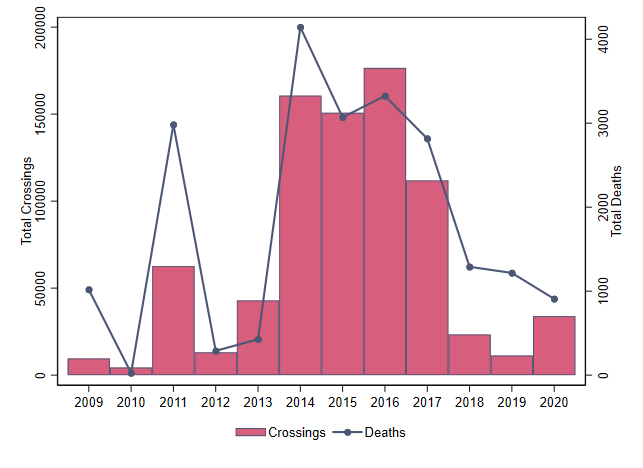
\includegraphics[width=0.75\textwidth]{../graphs/fig1.png}
\floatfoot*{\footnotesize Note: Bars show the total number of crossings to Italy (on the left axis). Solid line displays the number of deaths in transit along the Central Mediterranean Route (on the right axis). Italian data on total crossings come from the \emph{Polizia di Stato}, the Italian State Police. The data on deaths at sea are from The Migrants File data available at \url{https://www.themigrantsfiles.com}. The majority of the migrants over the Central Mediterranean route arrived to Italy (and a very small number to Malta). Over the same period Malta registered 24,778 total crossings only.}}
\end{figure}


\clearpage
\begin{table}[th!]\small
\RawCaption{\caption{EU Operations}\label{fig:tabpolicy}}
\floatbox[{\captop}]{table}[\FBwidth] 
{}
{\resizebox{\textwidth}{!}{\begin{tabular}{L{5cm}L{4cm}C{3.5cm}cc}
\toprule\toprule
&&Maritime SAR &\multicolumn{2}{c}{Budget}  \\
EU Operations     & Dates   &  Distance from Italian shores (in km) & per month & total \\
\hline
&&&&   \\
\textbf{Hermes - Main operations}          
& 16 Apr -- 16 Oct 09     & 44             & 0.9   & 5.2  \\
& 14 Jun \: -- 29 Oct 10     & 44             & 0.8     & 3.3  \\
& 20 Feb \: -- 31 Aug 11     & 44             & 2.5     & 15.0   \\
& 02  Jul \:  -- 30 Oct 12     & 44             & 1.0 & 4.1     \\
& 06  May -- 07 Oct 13     & 44             & 1.5 & 9.0    \\
\textit{Extension} & 01 Sep \: -- 31 Mar 12 & 22*             &     &  \\
\textit{Extension} & 01 Nov \: -- 31 Jan 13 & 22*             &   &    \\ 
\\
&\multicolumn{4}{c}{\textbf{Intense SAR}}  \\ \cline{2-5}
&                            &                &     &   \\
\textbf{Mare Nostrum}      & 18 Oct 13 -- 31 Oct 14     & 244            & 9.3  &  112  \\
&                            &                &   &     \\
\textbf{Triton I}         & 01 Nov 14 -- 30 Apr 15     & 56             & 2.9  & 27.5  \\
\textbf{Triton II}        & 01 May 15 -- 31 Jan 18       & 256            & 18.2   & 437  \\
&                              &                &    &    \\
\textbf{Themis}        	 & 01 Feb 18 -- 31 Dec 20       & 24            & 22.3   & 721  \\
&                            &                &     &   \\
\hline
&&Maritime SAR &\multicolumn{2}{c}{Fundraising}  \\
NGO Operations     & Dates   &  Op. Area & per month & total \\
\hline
&&& &  \\
MOAS              & 25 Aug -- 15 Oct 14     & Libyan shore    &  2.1    & 4    \\
MOAS              & 01 May -- 01 Oct 15     & Libyan shore      &  1.1  & 5.7      \\
MOAS              & 06 Jun -- 31 Dec 16     & Libyan shore & 0.86   & 6       \\
MOAS              & 01 Apr -- 01 Sep 17     & Libyan shore &  0.55  & 3.3      \\
&                              &                &    &    \\
&\multicolumn{4}{c}{\textbf{NGO code of conduct}}  \\ \cline{2-5}
\textbf{Minniti}         & 07 Aug 17 --      & 24             &  &  \\
&                              &                &    &    \\
\bottomrule\bottomrule
\end{tabular}%

\floatfoot*{\footnotesize Note: Budget numbers are in millions of Euro. More intense SAR operations are \emph{Mare Nostrum}, \emph{Triton I}, \emph{Triton II} and \emph{Themis}. Information on the extent of the SAR zone is sometimes hidden in official Frontex Operational Plans (2009-2020). Information on \emph{Mare Nostrum} and \emph{Triton I} are gathered from a report by Italian Parliament(\citeyear{MoD_2013}) and \citet{MoD_2015}. The 2016 and 2018 Frontex budgets provide details on Joint Operations \citep{Frontex_bud2016,Frontex_bud2018}. Budget during Themis Operation is retrieved from the Frontex Programming Document 2020 - 2022 \citep{Frontex_pd2019}. In these instances our best guess (*) is that surveillance occurred within the territorial sea, as defined by the 1982 United Nations Convention on the Law of the Sea (12 nautical miles, or 22 km from the coastal state).}}}
\end{table}


\clearpage
\begin{figure}[th!]\centering
	\RawCaption{\caption{Types of Vessels Used, 2013-2020}\label{transp}}  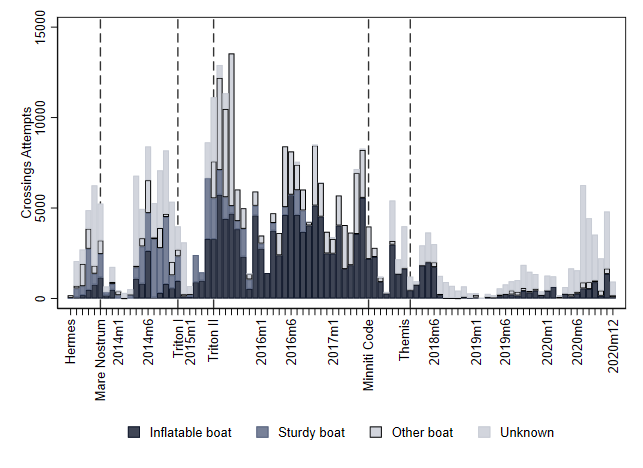
\includegraphics[width=.85\linewidth]{../graphs/fig2.png}
	\floatfoot*{\footnotesize Note: Bars show the monthly total number of crossings attempts to Italy by different types of boats. The information on crossing attempts, which are the sum of crossings and deaths in transit, are disclosed by the European Border and Coast Guard Agency known as Frontex (for the period from 1 January 2013 to October 2017) and by State Police (for the period November 2017 to December 2020). Vertical dotted lines display the start of SAR Operations (Hermes, Mare Nostrum, Triton I, II and Themis) and Minniti Code  (August 7, 2017).}	
\end{figure}


\clearpage
\begin{figure}[th!]\centering
	\RawCaption{\caption{Attempted Crossings by Ports of Departure, 2016-2020}\label{fig:raw}}
	\begin{tabular}{cc}
		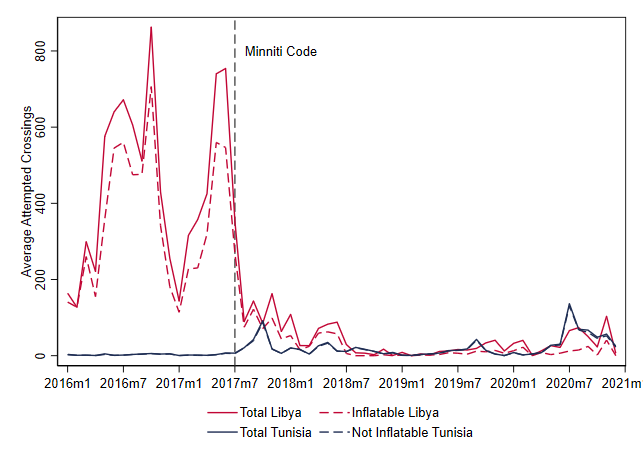
\includegraphics[width=.9\linewidth]{../graphs/fig3.png}
	\end{tabular}
	\floatfoot*{\footnotesize Note: Red and dark navy blue solid lines display the average attempted crossings by the month and the routes: Libya and Tunisia, respectively. Red and dark navy blue dashed lines display the average attempted crossings with inflatables. The information on crossing attempts, which are the sum crossings and deaths in transit, by different routes (Libya  and Tunisia) and types of boats (Inflatable and Not Inflatable boats) are disclosed by \emph{Polizia di Stato}, the Italian State Police (2016-2020). Vertical dotted lines display the start of Minniti Code (August 7, 2017).}
\end{figure}



\clearpage
\begin{figure}[th!]\centering
\RawCaption{\caption{Predicted Points of Departure, 2011-2017}\label{fig:angle}} 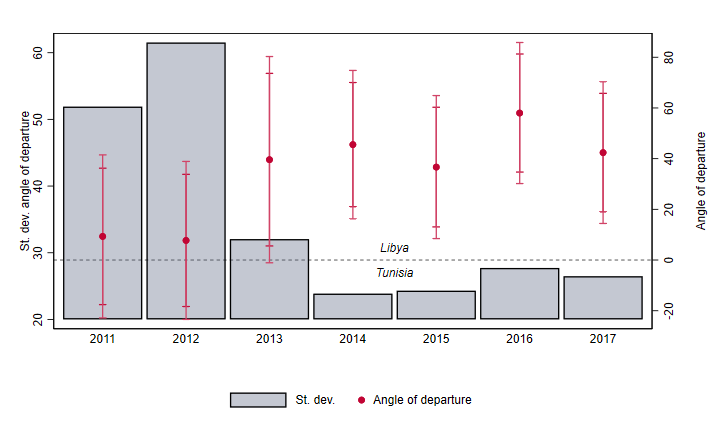
\includegraphics[width=.85\textwidth]{../graphs/fig4.png}		
\floatfoot*{\footnotesize Note: The figure shows the average angle of departure based on the locations of shipwrecks and corresponding 90 and 95 percent confidence intervals. The total number of observations is 143. The angles are normalized so that negative values correspond to predicted departures from Tunisia and positive values correspond to predicted departures from Libya. See Appendix Figure \ref{fig:angle2} for a detailed map of shipwrecks used to construct this figure.} 	
\end{figure}
	

\clearpage	
\begin{table}[th!]\small
	\RawCaption{\caption{Summary Statistics}\label{tab:sum}}
	\floatbox[{\captop}]{table}[\FBwidth]
	{}
	{\resizebox{\textwidth}{!}{\begin{tabular}{L{10cm}C{2cm}C{2cm}C{2cm}C{2cm}}
\toprule\toprule
\multicolumn{5}{c}{\textbf{Sample 2013-2017: 1612 Observations}}                        \\
& \textit{Mean}    & \textit{Sd}      & \textit{Min}   & \textit{Max}   \\
	                                 &         &         &       &       \\
Attempted Crossings                          & 164.483 & 316.160 & 0     & 3051  \\
Wave Height in Tripoli \textit{(33$^\circ$N 13$^\circ$30$^\prime$E) }  				& 0.787   & 0.498   & 0.108 & 4.164 \\
Max Wave Height in Tripoli (t,t-1)                  						& 0.926   & 0.568   & 0.143 & 4.164 \\
Wave Height in Zuwara \textit{(33$^\circ$N 12$^\circ$00$^\prime$E)}    				& 0.671   & 0.376   & 0.101 & 3.071 \\
Wave Height in Al Huwariyah \textit{(37$^\circ$25$^\prime$N 11$^\circ$25$^\prime$E)} & 1.015   & 0.743   & 0.070 & 5.274 \\
Wave Height in Monastir \textit{(36$^\circ$N 11$^\circ$25$^\prime$E)} 				& 0.865   & 0.601   & 0.073 & 4.173 \\
Wave Height in Djerba  \textit{(34$^\circ$N 11$^\circ$00$^\prime$E)}  				& 0.746   & 0.434   & 0.084 & 2.848 \\
Wave Height in Annaba \textit{(37$^\circ$5$^\prime$N 7$^\circ$30$^\prime$E)}    		& 0.966   & 0.727   & 0.145 & 5.580 \\
Fraction of Inflatable Boats                 & 0.395   & 0.374   & 0     & 1     \\
Fraction of Inflatable+Unknown Boats         & 0.586   & 0.422   & 0     & 1     \\
Fraction of Inflatable+Unknown+Other Boats & 0.656   & 0.396   & 0     & 1     \\
\toprule\toprule
	                                 &         &         &       &       \\
\multicolumn{5}{c}{\textbf{Sample 2016-2020:   3654 Observations (1827 by Route)}}        \\
& \textit{Mean}    & \textit{Sd}      & \textit{Min}   & \textit{Max}   \\
Route: \textbf{Lybia}                                 &         &         &       &       \\
\cline{1-1}
Attempted Crossings                          & 168.547 & 511.015 & 0     & 5504  \\
Wave Height                                  & 0.928   & 0.618   & 0.120 & 5.506 \\
Fr. of Inflatable Boat                       & 0.474   & 0.398   & 0     & 1     \\
&         &         &       &       \\
Route: \textbf{Tunisia}                               &         &         &       &       \\
\cline{1-1}
Attempted Crossings                          & 17.284  & 51.733  & 0     & 580   \\
Wave Height                                  & 0.786   & 0.588   & 0.091 & 4.403 \\
Fraction of Inflatable Boats                 & 0.119   & 0.258   & 0     & 1     \\
\bottomrule\bottomrule 
\end{tabular}%





% The wave height at Annaba (Algeria) is measured at 37.5N 7 30E. 
% The location in Al Huwariyah (37.25, 11.25) 
% while Monastir has latitude 36 and longitude 11.25 





			\floatfoot*{\footnotesize Note: The two subsamples consist of daily crossings from 1 January 2013 to 31 December 2017 and daily crossings disaggregated by country of departure (Libya and Tunisia) from 1 January 2016 to 31 December 2020. Crossing attempts include successful crossings and deaths in transit. Significant wave height is measured in meters and in different locations: Tripoli and Zuwara, Libya; Al Huwariyah, Monastir and Djerba, Tunisia; Annaba, Algeria. The data on wave height come from the European Centre for Medium-Range Weather Forecasts (ECMWF) from daily runs at 12 UTC.  The spatial resolution of the data set is approximately 79 km spacing for the surface around the geographical coordinates.
			}
	}}
\end{table}	


	
	\begin{figure}[b!]\centering
		\begin{center}
			\protect\caption{Migrant's Crossing Decisions}\label{fig:migrants}
			
			\centering 		
			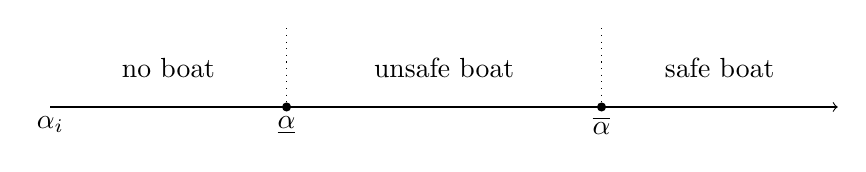
\begin{tikzpicture}[xscale=10,yscale=10]
			\draw [->] (0,0) -- (1,0);
			\node [below] at (0,0) {$\alpha_i$};
			
			\node [below,black] at (0.3,0) {$\underline{\alpha}$};
			\draw [fill, black] (0.3,0) circle[radius=0.005];
			
			\node [below,black] at (0.7,0) {$\overline{\alpha}$};
			\draw [fill,black] (0.7,0) circle[radius=0.005];
			\draw [dotted] (0.3,0.1) -- (0.3,0);
			\draw [dotted] (0.7,0.1) -- (0.7,0);
			
			\node  at (0.15,0.05) {no boat};
			\node at (0.5,0.05) {unsafe boat};
			\node  at (0.85,0.05) {safe boat};
			
			\end{tikzpicture}
		\end{center}
	\end{figure}
	

\clearpage
\begin{figure}[th!]\centering
	\begin{center}
		\protect\caption{\emph{Ex Ante} Crossing Risk}\label{fig:crossing risk}
		
		\centering 		
		\begin{tikzpicture}[xscale=7,yscale=7]
		\draw [->] (0,0) -- (1,0);
		\draw [->] (0,0) -- (0,0.7);
		\node [left] at (1.10,0) {$\sigma_u$};
		\node [above] at (0,0.75) {$\rho$};
		\node [left] at (0,0.3) {1-$\sigma_s$};
		\node [below] at (0,0) {0};
		\node [below] at (0.7,0) {$\sigma_s$};
		
		\draw [dotted] (0,0.3) -- (0.7,0.3);
		\draw [dotted] (0.7,0) -- (0.7,0.3);
		
		\draw plot [smooth] coordinates {(0,0.3) (0.2,0.45) (0.4,0.53) (0.6,0.4) (0.7,0.3) (0.95,0.05)};		
		\end{tikzpicture}
	\end{center}
\end{figure}


	
	\begin{figure}[b!]\centering
	\begin{center}
		\protect\caption{Incidence of Search and Rescue Operations on Migrants}\label{fig:incidence migrants}
		\captionsetup[subfloat]{labelformat=empty, labelsep=none, position=top}
		\subfloat[(a) Perfect Competition]{
			\centering 		
			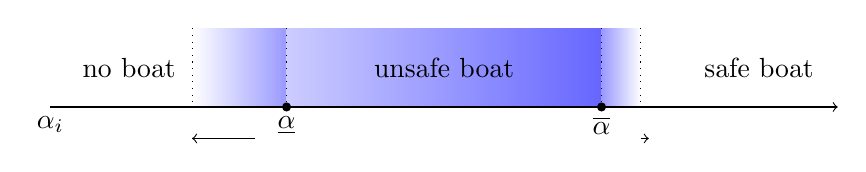
\begin{tikzpicture}[xscale=10,yscale=10]		
			\fill[left color = white,right color = blue!40] (0.18,0) rectangle (0.3,0.1);
			\fill[left color = blue!20,right color = blue!60] (0.3,0) rectangle (0.7,0.1);		
			\fill[left color = blue!40,right color = white] (0.7,0) rectangle (0.75,0.1);
			
			\draw [->] (0,0) -- (1,0);
			\node [below] at (0,0) {$\alpha_i$};
			
			\node [below,black] at (0.3,0) {$\underline{\alpha}$};
			\draw [fill, black] (0.3,0) circle[radius=0.005];
			
			\node [below,black] at (0.7,0) {$\overline{\alpha}$};
			\draw [fill,black] (0.7,0) circle[radius=0.005];
			
			\draw [dotted] (0.3,0.1) -- (0.3,0);
			\draw [dotted] (0.7,0.1) -- (0.7,0);
			
			\draw [->] (0.26,-0.04) -- (0.18,-0.04);
			\draw [dotted] (0.18,0.1) -- (0.18,0);
			
			\draw [->]  (0.75,-0.04) -- (0.76,-0.04);
			\draw [dotted] (0.75,0.1) -- (0.75,0);
			
			\node at (0.1,0.05) {no boat};
			\node at (0.5,0.05) {unsafe boat};
			\node at (0.9,0.05) {safe boat};
			\end{tikzpicture}}
		
		\subfloat[(b) Monopolist Smuggler]{
			\centering
			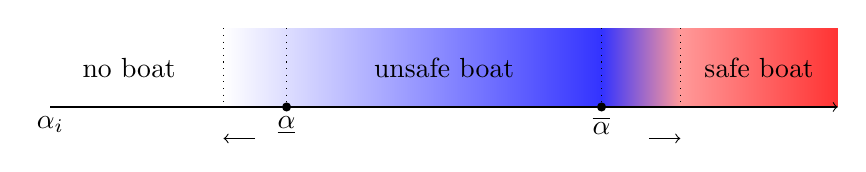
\begin{tikzpicture}[xscale=10,yscale=10]
			\fill[left color = white,right color = blue!80] (0.22,0) rectangle (0.7,0.1);
			\fill[left color = blue!80, right color = red!40] (0.7,0) rectangle (0.8, 0.1);
			\fill[left color = red!40,right color = red!80] (0.8,0) rectangle (1,0.1);
			\draw [->] (0,0) -- (1,0);
			\node [below] at (0,0) {$\alpha_i$};
			
			\node [below,black] at (0.3,0) {$\underline{\alpha}$};
			\draw [fill, black] (0.3,0) circle[radius=0.005];
			
			\node [below,black] at (0.7,0) {$\overline{\alpha}$};
			\draw [fill,black] (0.7,0) circle[radius=0.005];
			
			\draw [dotted] (0.3,0.1) -- (0.3,0);
			\draw [dotted] (0.7,0.1) -- (0.7,0);
			
			\draw [->] (0.26,-0.04) -- (0.22,-0.04);
			\draw [dotted] (0.22,0.1) -- (0.22,0);
			
			\draw [->] (0.76,-0.04) -- (0.80,-0.04);
			\draw [dotted] (0.80,0.1) -- (0.80,0);
			
			\node at (0.1,0.05) {no boat};
			\node at (0.5,0.05) {unsafe boat};
			\node at (0.9,0.05) {safe boat};
			\end{tikzpicture}}
		
		\floatfoot{\footnotesize Note: The blue region contains migrants who are made better off by search and rescue operations, and the red region contains migrants who are made worse off by search and rescue operations. A greater intensity of color reflects a greater (positive or negative) incidence.}
	\end{center}
\end{figure}



\clearpage 
\begin{table}[th!]\small
\RawCaption{\caption{Elasticities of Crossing Attempts to Crossing Conditions}\label{tab:boats_migrants}}
\floatbox[{\captop}]{table}[\FBwidth]
{}
{\resizebox{\textwidth}{!}{ \begin{tabular}{p{7cm}C{3.5cm}C{3.5cm}C{3.5cm}} \toprule\toprule         & (1)   & (2)   & (3)   \\         
 & \multicolumn{3}{c}{\textbf{Crossing Attempts}}                                          \\         \hline           
                    &            &            &            \\ 
 & \multicolumn{3}{c}{\textbf{Definition of Unsafe Boat}} \\   
       \cline{2-4}      & \textit{Inflatable} & \textit{Inflatable +} & \textit{Inflatable +} \\         & \textit{} & \textit{Unknown} & \textit{Unknown +}  \\         & \textit{} & \textit{} & \textit{Other}  \\         \hline                 
                    &            &            &            \\
Wave Height * Post SAR * Fr. Boat&      -6.546&      -5.450&      -4.168\\
                    &     (1.929)&     (1.397)&     (1.293)\\
Wave Height         &      -0.891&      -1.430&      -1.458\\
                    &     (0.366)&     (0.605)&     (0.612)\\
Wave Height * Fr. Boat&       2.135&       1.907&       1.632\\
                    &     (1.813)&     (1.342)&     (1.131)\\
Wave Height * Post SAR&       0.209&       1.165&       1.004\\
                    &     (0.455)&     (0.647)&     (0.727)\\
         \midrule Week-Year FE & \checkmark & \checkmark & \checkmark  \\ {\it Pre SAR Period Statistics} &  &  &   \\ Mean Total Attempt  & 120 & 120 & 120 \\ Mean Wave Height  & .63 & .63 & .63 \\ Mean Frac. Unsafe Boat  & .07 & .27 & .29 \\         
Observations        &        1612&        1612&        1612\\
         \bottomrule         \end{tabular}         

\floatfoot*{\footnotesize Note: The sample consists of daily observations from 7 May 2013 to 4 October 2017. SAR coefficients are estimated relative to a baseline in which Hermes operations (single boat type regime) were in place (164 days). Post SAR dummy is equal to one for all observations after October 18, 2013 (the beginning of the intense SAR, when multiple boat types were used).  Crossing attempts sum crossings and deaths in transit. Significant wave height in Tripoli (Libya) is measured in meters. Frac. Unsafe Boat measures the share of attempted crossings using unsafe boats aggregated at the week-year level. We define three different categories of unsafe boats based on the main vessels used. The share of crossing attempts using ``inflatable'' rubber boats over the total; we then add the ``unknown boats'' and ``other boats'', excluding any sturdy and motor boats. All regressions control for week-by-year fixed effects. Regressions are estimated using Poisson quasi-maximum likelihood models. Standard errors are heteroscedasticity- and autocorrelation-robust using Newey-West with a bandwidth equal to 28 days.
}}}
\end{table}	


\clearpage 
\begin{table}[t!]\small
	\RawCaption{\caption{Elasticities of Crossing Attempts to Crossing Conditions by Country of Departure}\label{tab:did}}
	\floatbox[{\captop}]{table}[\FBwidth]
	{}
	{\resizebox{\textwidth}{!}{ \begin{tabular}{p{11.5cm}C{3cm}C{3cm}} \toprule\toprule         & (1)   & (2)      \\         & \multicolumn{2}{c}{\textbf{Crossing Attempts}}                                          \\         \hline &            &                                \\                 
SAR $\times$ From Libya&       4.411&            \\
                    &     (0.202)&            \\
From Libya          &       0.503&            \\
                    &     (0.124)&            \\
Wave   Height       &            &      -2.295\\
                    &            &     (0.376)\\
Wave   Height $\times$ Frac. Inflatable Boat&            &      -2.374\\
                    &            &     (2.774)\\
SAR $\times$ Wave   Height&            &      -0.764\\
                    &            &     (0.726)\\
SAR $\times$ Wave   Height $\times$ Frac. Inflatable Boat&            &       4.015\\
                    &            &     (3.177)\\
From Libya $\times$ Wave   Height&            &       1.807\\
                    &            &     (0.729)\\
From Libya $\times$ Wave   Height $\times$ Frac. Inflatable Boat&            &       2.316\\
                    &            &     (2.867)\\
From Libya $\times$ SAR $\times$ Wave   Height&            &       2.821\\
                    &            &     (1.647)\\
From Libya $\times$ SAR $\times$ Wave   Height $\times$ Frac. Inflatable Boat&            &      -6.974\\
                    &            &     (3.707)\\
         \midrule Week-Year FE & \checkmark &    \\ Week-Year-From Lybia FE & & \checkmark   \\         
Observations        &        3402&        2952\\
         \bottomrule         \end{tabular}         

\floatfoot*{\footnotesize Note: The sample consists of daily observations from 1 January 2016 to 31 December 2020. SAR dummy is equal to one for all observations before August 7, 2017, when multiple boat types were used more frequently. This corresponds to pre-\emph{Minniti} periods, i.e.~before the Code of Conduct was enacted restricting \textit{de-facto} the use of unsafe boats. Crossing attempts sum crossings and deaths in transit. Significant wave height is measured in meters in Tripoli, Libya and Tunis, Tunisia depending on the departure location. The dummy ``From Libya'' takes value one if the migrants departed from Libya (treated units). Frac. Inflatable Boat measures the share of attempted crossings using inflatable boats aggregated at the week-year level. Crossing attempts sum crossings and deaths. In column 1 we control for week-by-year fixed effects. In column 2 we add the interaction with the dummy ``From Libya'', causing a drop in observations (450) because of zero attempted crossings both from Libya and Tunisia. Regressions estimated using Poisson quasi-maximum likelihood models. Standard errors are cluster at the week of the year level.
				}}}
\end{table}	


\begin{figure}[t!]\centering
	\RawCaption{\caption{Simulated Probability of Success on Unsafe Boat vs. Safe Boat by Relative Price \label{fig:teta}}}
	\begin{tabular}{cc}
		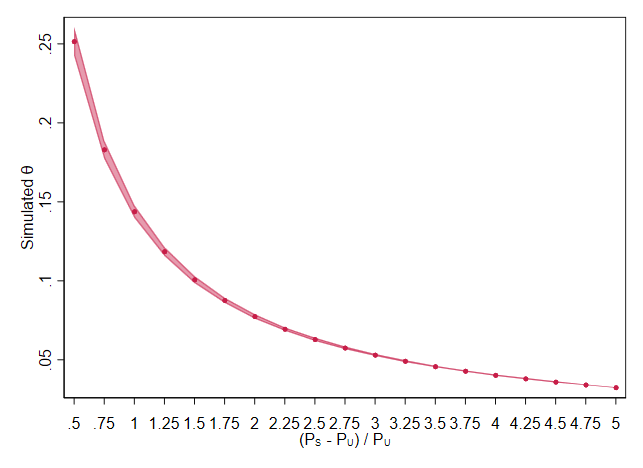
\includegraphics[width=.7\linewidth]{../graphs/fig8.png}
	\end{tabular}
	\floatfoot{\footnotesize Note: The $\hat{\theta} = \frac{\sigma_U}{\sigma_S}$s are simulated using the semi-elasticities estimated in Column (1) of Table \ref{tab:boats_migrants}. 95\% confidence intervals are shown with standard errors computed using the $\delta$-method. }
\end{figure}





\begin{table}[b!]\small 
	\RawCaption{\caption{Fraction of Migrants by Boat Types}\label{tab:boatsA}}
	\floatbox[{\captop}]{table}[\FBwidth]
	{}
	{\resizebox{\textwidth}{!}{ \begin{tabular}{p{5cm}C{3cm}C{3cm}C{3cm}C{3cm}C{3cm}} \toprule\toprule   & (1)         & (2)       & (3)     & (4)      & (5)       \\ Fraction of Attempted Crossings       & Inflatable   & Inflatable + & Inflatable + & Fishing & Motor                     \\                                            &    & Unknown & Unknown + &  &                      \\                                            &    &  & Other &  &                      \\ \hline                          &        &       &          &     &                           \\ 
Mare Nostrum        &       0.058&      -0.066&       0.099&       0.052&      -0.151\\
                    &     (0.047)&     (0.065)&     (0.078)&     (0.065)&     (0.065)\\
Triton I            &       0.303&       0.142&       0.316&       0.037&      -0.353\\
                    &     (0.103)&     (0.089)&     (0.083)&     (0.072)&     (0.081)\\
Triton II           &       0.606&       0.545&       0.532&      -0.165&      -0.367\\
                    &     (0.037)&     (0.049)&     (0.050)&     (0.044)&     (0.052)\\
         \midrule Pre MN Mean Outcome  & .11 & .38 & .42 & .22 & .36 \\         
Observations        &         768&         768&         768&         768&         768\\
         \bottomrule         \end{tabular}         
 
			\floatfoot*{\footnotesize Note: The sample consists of daily observations from 7 May 2013 to 4 October 2017. SAR coefficients are estimated relative to a baseline in which Hermes operations were in place (164 days). More intense SAR (i.e. Mare Nostrum  (MN), Triton I and II) dummies are equal to one over the periods defined in Table \ref{fig:tabpolicy}. We show the fractions of attempted crossings  using ``inflatable'' rubber boats over the total; adding the category ``unknown boats'' and then the ``other boats''. Last two columns show the fraction of attempted crossings  using sturdy boats, i.e. fishing and motor boats, respectively. All regressions control for 52 weeks of the year fixed effects. The 768 observations correspond to days with at least one crossing during SAR periods. Regressions estimated using OLS. Cluster standard errors at the weekly level.
				}}}
\end{table}	



\clearpage 
\begin{figure}[th!]\centering
	\RawCaption{\caption{Fraction of Inflatable Boats around the Introduction of the ``Minniti Code''}\label{fig:minniti}}
	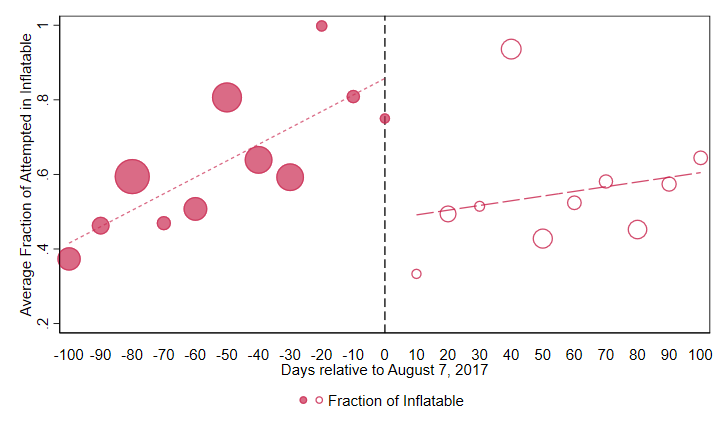
\includegraphics[width=.8\linewidth]{../graphs/fig9.png}	
	\floatfoot*{\footnotesize Note: The Minniti Code of Conduct was introduced on the August 7, 2017. Circle size is proportional to the number of attempted crossings.}
\end{figure}


\clearpage
	
	\newpage
	\bibliographystyle{elsarticle-harv}
	\bibliography{references}
	
	\newpage
	\appendix
	
	
%%%%%%%%%%%%%%%%%%%%%%%%%%%%%%%%%%%%%%%%%%%%%%%%%%%%%%%%%%%%%%%%%%%%%%%%%
\setcounter{section}{0} \renewcommand{\thesection}{A}
\setcounter{subsection}{0} \renewcommand{\thesubsection}{A.\arabic{subsection}}
\setcounter{figure}{0} \renewcommand{\thefigure}{A.\arabic{figure}}
\setcounter{table}{0} \renewcommand{\thetable}{A.\arabic{table}}
	
\clearpage
\section*{Appendix A: Institutional Background}



\begin{figure}[th!]\centering
\RawCaption{\caption{Percentage of Migrants Intercepted at Sea by Libyan and Italian Coast Guards} \label{LCG}}
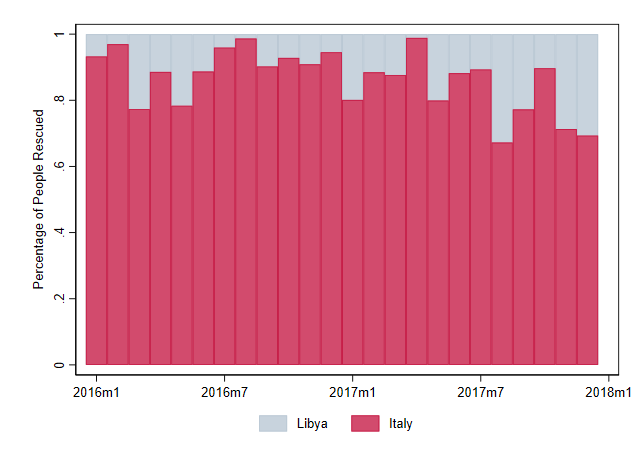
\includegraphics[width=.8\linewidth]{../graphs/figA1.png}
\floatfoot*{\footnotesize Note: Data are from the United Nations High Commissioner for Refugees (UNHCR, 2017) that provides the monthly number of migrants intercepted at sea by the coast guards. Red and grey bars show the percentages of the people rescued by Libyan and Italian coast guards, respectively.}
\end{figure}




\clearpage

\section*{Appendix C: Additional Tables and Figures}
\setcounter{subsection}{0} 	
\renewcommand{\thesubsection}{C.\arabic{subsection}}
\setcounter{figure}{0} 		
\renewcommand{\thefigure}{C.\arabic{figure}}
\setcounter{table}{0}  		
\renewcommand{\thetable}{C.\arabic{table}}


\begin{figure}[th!]\centering
\RawCaption{\caption{Nationalities of Migrants on the Central Route by Year}\label{national}}	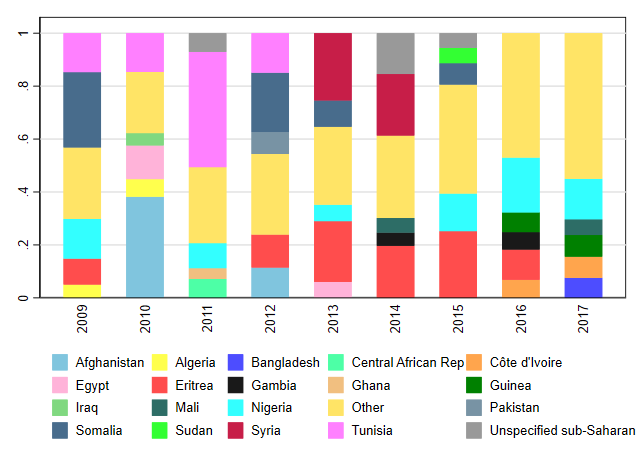
\includegraphics[width=.8\linewidth]{../graphs/figC1.png}
\floatfoot*{\footnotesize Note: Data are collected by the European Border and Coast Guard Agency and are based on detections at the border. Our subset is based on detections along the Central Mediterranean Route and the figures show the fraction of detections for the top six nationality from 2009 to 2017.}
\end{figure}

%%%%%%%%%%%%%%%%%%%%%%%%%%%%%%%%%%%%%%%%%%%%%%%%%%%%%%%%%%%%%%%%%%%%%%%%%%%%%%%%%%%%%%%%%%%%%%%%%%%%%%%%%%%%%%%%%%%%%
\clearpage
\begin{figure}[th!]\centering
	\RawCaption{\caption{Monthly Crossing Attempts}\label{tot_sbar_ym}}	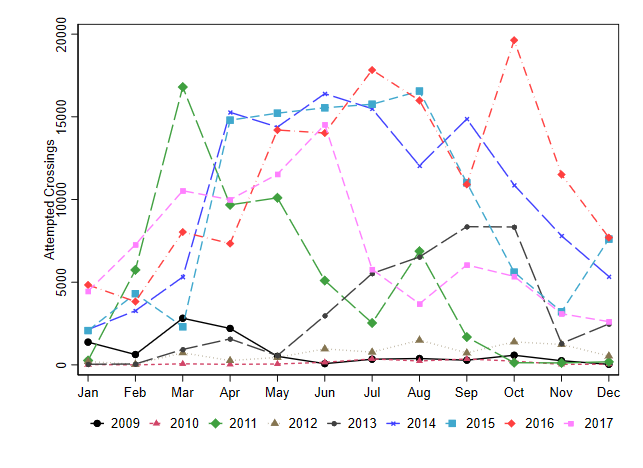
\includegraphics[width=.8\linewidth]{../graphs/figC2.png}
	\floatfoot*{\footnotesize Data on crossings are provided by \emph{Polizia di Stato}, the Italian State Police. Data on deaths at sea are described in  Section \ref{s:UNITED}. The figure shows the total number of monthly crossing attempts that sum the crossings and the deaths in transit.}
\end{figure}

%%%%%%%%%%%%%%%%%%%%%%%%%%%%%%%%%%%%%%%%%%%%%%%%%%%%%%%%%%%%%%%%%%%%%%%%%%%%%%%%%%%%%%%%%%%%%%%%%%%%%%%%%%%%%%%%%%%%%
\clearpage
\begin{figure}[th!]\centering
\RawCaption{\caption{Net-Imports of Rubber Boats, Wooden Ferries and Life Jackets}\label{diffindiff}} \begin{tabular}{cc}
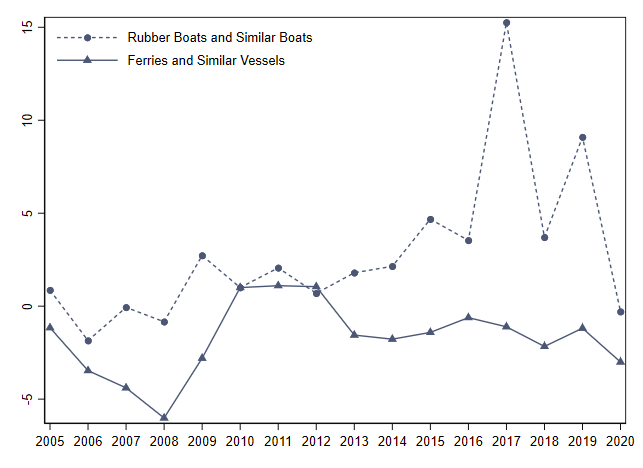
\includegraphics[width=.45\linewidth]{../graphs/figC3a.png}		
&
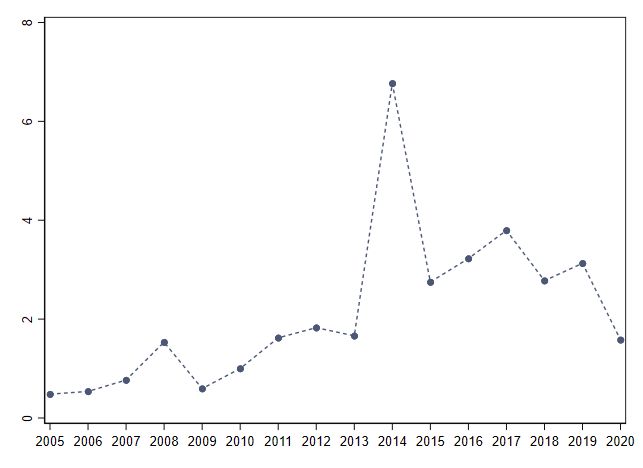
\includegraphics[width=.45\linewidth]{../graphs/figC3b.png}	\\
Rubber Boats, Wooden Ferries & Life Jackets \\
\end{tabular}
\floatfoot*{\footnotesize Note: Data come from UN Comtrade  over the period 2005-2020. The series show net-imports of rubber boats and ferries (left panel) and Life Jackets (right panel) to countries near Libya for which data are available (Malta, Turkey, and Egypt). Both series are normalized to 1 in 2010.}
\end{figure}


%%%%%%%%%%%%%%%%%%%%%%%%%%%%%%%%%%%%%%%%%%%%%%%%%%%%%%%%%%%%%%%%%%%%%%%%%%%%%%%%%%%%%%%%%%%%%%%%%%%%%%%%%%%%%%%%%%%%%
\clearpage
\begin{figure}[th!]\centering
	\RawCaption{\caption{Map of Angles}\label{fig:angle2}}
	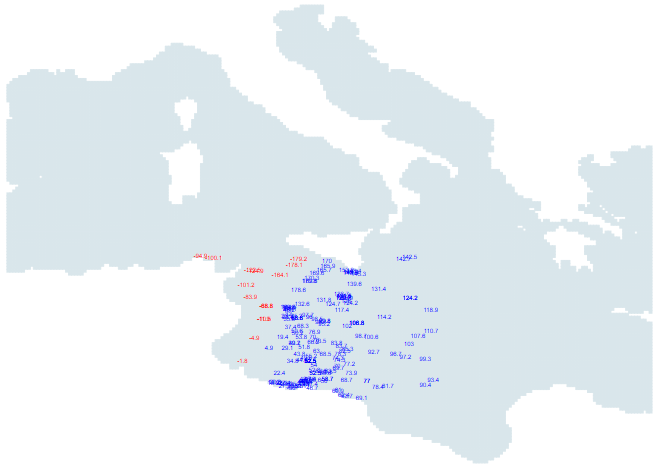
\includegraphics[width=1\textwidth]{../graphs/figC4.png}
	\floatfoot*{\footnotesize Note: The figure shows the location of shipwrecks and the corresponding angle with respect to Lampedusa. The angle is normalized to be zero between Lampedusa and the shore at the border between Tunisia and Libya, close to the island of Djerba. The angle becomes more negative moving west towards Tunisia and more positive moving East towards Libya. The total number of observations is 143.}	
\end{figure}



%%%%%%%%%%%%%%%%%%%%%%%%%%%%%%%%%%%%%%%%%%%%%%%%%%%%%%%%%%%%%%%%%%%%%%%%%%%%%%%%%%%%%%%%%%%%%%%%%%%%%%%%%%%%%%%%%%%%%
\clearpage
\begin{table}[th!]\small
	\RawCaption{\caption{Irregular Migration During Search and Rescue Operations}\label{tab:SAR}}
	\floatbox[{\captop}]{table}[\FBwidth]
	{}
	{\resizebox{\textwidth}{!}{ \begin{tabular}{p{5cm}C{2.5cm}C{2.5cm}C{2.5cm}C{2.5cm}C{2.5cm}C{2.5cm}C{2.5cm}} \toprule\toprule   & (1)         & (2)    & (3)    & (4)    & (5)    & (6) & (7)         \\  & \textbf{Crossing Attempts} & Crossing Risk & \multicolumn{5}{c}{Distance (in km) to:} \\    \cline{4-8} &       &     &   Tripoli    &  Bengazi    & Al Huwariyah & Min (Tripoli & Lampedusa \\ &                                 &     &       &    & &  Bengazi \& &  \\  & &     &       &    & &  Al Huwariyah) &  \\ \hline           &       &     &       &    &  &&  \\                 
Hermes 2011         &       2.214&       0.003&     -34.195&     -49.703&      38.009&      -5.162&       0.707\\
                    &     (0.381)&     (0.029)&    (28.781)&    (21.430)&    (27.196)&    (20.709)&    (25.131)\\
Hermes 2011a        &      -0.261&       0.033&     -32.633&    -120.588&     120.099&      37.411&      66.968\\
                    &     (0.491)&     (0.049)&    (32.877)&    (47.014)&    (58.849)&    (26.820)&    (53.770)\\
Hermes 2012         &       0.230&       0.029&     -22.268&      -7.751&      -1.340&       5.570&     -32.664\\
                    &     (0.337)&     (0.020)&    (50.063)&    (42.103)&    (55.997)&    (27.392)&    (52.359)\\
Hermes 2013         &       1.700&       0.002&      47.337&     -61.759&      26.278&      95.944&     -17.002\\
                    &     (0.349)&     (0.021)&    (38.765)&    (36.189)&    (34.143)&    (21.385)&    (31.530)\\
Hermes 2013a        &       0.490&       0.059&     -47.906&     -20.130&      44.605&     -19.753&      16.760\\
                    &     (0.502)&     (0.057)&    (26.483)&    (28.599)&    (29.925)&    (18.823)&    (26.472)\\
Mare Nostrum        &       2.554&       0.070&    -107.554&    -106.336&     123.249&     -29.174&      66.636\\
                    &     (0.301)&     (0.027)&    (33.611)&    (22.857)&    (28.027)&    (25.077)&    (21.065)\\
Triton I            &       2.420&       0.076&    -180.596&    -102.924&     160.504&     -63.948&      83.784\\
                    &     (0.371)&     (0.032)&    (26.518)&    (25.916)&    (25.704)&    (17.959)&    (16.501)\\
Triton II           &       2.564&       0.101&    -171.165&    -101.383&     167.246&     -77.340&     106.632\\
                    &     (0.292)&     (0.020)&    (25.274)&    (18.767)&    (23.673)&    (15.815)&    (17.137)\\
         \midrule Week FE & \checkmark & \checkmark & \checkmark & \checkmark & \checkmark & \checkmark & \checkmark \\ {\it Pre SAR Period Statistics} &  &  & &  &  & &  \\ Pre Mean Outcome & 24 & .03 & 326 & 784 & 259 & 206 & 135 \\         
Observations        &        3287&        1579&         503&         503&         503&         503&         503\\
         \bottomrule         \end{tabular}         
   
			\floatfoot*{\footnotesize Note: The sample in column (1) consists of daily observations from 1 January 2009 to 31 December 2017 (3,287). The sample in column (2) consists of daily observations from 1 January 2009 to 31 December 2017 (1,579), i.e. when deaths and total attempts are simultaneously different from zero. The sample in column (3)-(7) consists of 503 geo-localized rescue events from 18 January 2009 to 22 December 2017. SAR coefficients (Hermes, Mare Nostrum, Triton I and II) are estimated relative to the baseline period in which no SAR operations were in place. Crossing attempts sum crossings and deaths in transit. Significant wave height in Tripoli (Libya) is measured in meters. Crossing Risk is defined as the number of deaths over total attempts. Distances, expressed in Km, measures the shortest linear distance between different locations (Tripoli, Bengazi (Libya), Al Huwariyah (Tunisia) and Lampedusa (Italy) and the latitude and the longitude of the casualties at sea. All regressions control for 52 weeks of the year fixed effects. Regressions estimated with PPML and OLS. Standard errors clustered by month of the year }}}
\end{table}


%%%%%%%%%%%%%%%%%%%%%%%%%%%%%%%%%%%%%%%%%%%%%%%%%%%%%%%%%%%%%%%%%%%%%%%%%%%%%%%%%%%%%%%%%%%%%%%%%%%%%%%%%%%%%%%%%%%%%
\clearpage
\begin{table}[th!]\small
	\RawCaption{\caption{Wave and Swell Explanations}\label{tab:waveswell}}
	\floatbox[{\captop}]{table}[\FBwidth]
	{}
	{\resizebox{\textwidth}{!}{\documentclass[class=article,crop=true]{standalone}
%\usepackage{fullpage}
\usepackage{tikz}								%create timelines
	\usetikzlibrary{arrows,backgrounds,snakes}
\usepackage{amsmath}
\usepackage{pifont}
\newcommand{\cmark}{\ding{51}}%
\newcommand{\xmark}{\ding{55}}%
\usepackage{amsfonts}
\usepackage{amssymb}
\usepackage{graphicx}
\usepackage{adjustbox}
\usepackage{graphicx}
\usepackage{caption} 
\captionsetup[table]{skip=10pt}
\usepackage[capposition=top]{floatrow}			%to add notes on floats
\usepackage{siunitx}
\usepackage{float}								%package for layout of floats (tables, figures, etc.)
\floatstyle{plaintop}							%caption above the body of the float
\restylefloat{figure}							%apply float style to figures
\restylefloat{table}							%apply float style to tables
\usepackage{multirow}
\usepackage{array}
	\newcolumntype{L}[1]{>{\raggedright\let\newline\\\arraybackslash\hspace{0pt}}m{#1}}
	\newcolumntype{C}[1]{>{\centering\let\newline\\\arraybackslash\hspace{0pt}}m{#1}}
	\newcolumntype{R}[1]{>{\raggedleft\let\newline\\\arraybackslash\hspace{0pt}}m{#1}}
	
\begin{document}
 
\begin{tabular}{L{6cm}L{6cm}L{6.5cm}}
\toprule\toprule
   \textbf{Wave}: Description     & Height (metres)  &Effect          \\
  \hline
   Calm (rippled)                & 0.00   - 0.10          & No waves breaking                                                \\
   Smooth                               & 0.10 - 0.50        & Slight waves breaking                                            \\
   Slight                               & 0.50 - 1.25       & Waves rock buoys and small craft                                          \\
   Moderate                             & 1.25 - 2.50       & Sea becoming furrowed                                                     \\
   Rough                                & 2.50 - 4.00          & Sea deeply furrowed                                                       \\
   Very rough                           & 4.00 - 6.00          & Sea much disturbed with rollers                      \\
   High                                 & 6.00 - 9.00         & Sea disturbed with damage to foreshore \\
   Very high                            & 9.00 - 14.00         & Towering seas                                                             \\
   Phenomenal                           & \textgreater{}14 & Precipitous seas (only in cyclones)                           \\
   &                  &   
                                         \\
                                            \hline  \hline                                 
    \textbf{Swell}: Description                   & Wave Length   (metres)     & Wave Height  (metres)                                                               \\
     \hline
   Low swell of short or average length & 0 - 200        & 0 - 2                       \\
   Long, low swell                      & over 200       & 0 - 2                                                                    \\
   Short swell of moderate height       & 0 - 100          & 2 - 4                    \\
   Average swell of moderate height     & 100 - 200        & 2 - 4                        \\
   Long swell of moderate height        & over 200       & 2 - 4           \\
   Short heavy swell                    & 0 - 100          & over 4                                                                  \\
   Average length heavy swell           & 100 - 200        & over 4              \\
   Long heavy swell                     & over 200       & over 4     \\
\bottomrule\bottomrule
\end{tabular}%
\end{document}
			\floatfoot*{\footnotesize Note: The Bureau of Meteorology provides significant wave height that describes the combined height of the sea and the swell that mariners experience on open waters. See \url{http://www.bom.gov.au/marine/knowledge-centre/reference/waves.shtml}}
	}}
\end{table}
 

%%%%%%%%%%%%%%%%%%%%%%%%%%%%%%%%%%%%%%%%%%%%%%%%%%%%%%%%%%%%%%%%%%%%%%%%%%%%%%%%%%%%%%%%%%%%%%%%%%%%%%%%%%%%%%%%%%%%%
\clearpage
\begin{table}[th!]\small
	\RawCaption{\caption{Crossing Attempts: Robustness using OLS}\label{tab:boats_migrants_ols}}
	\floatbox[{\captop}]{table}[\FBwidth]
	{}
	{\resizebox{\textwidth}{!}{ \begin{tabular}{p{7cm}C{3.5cm}C{3.5cm}C{3.5cm}} \toprule\toprule         & (1)   & (2)   & (3)   \\         & \multicolumn{3}{c}{\textbf{Crossing Attempts}}                                          \\         \hline                         &            &            &            \\      & \multicolumn{3}{c}{\textbf{Definition of Unsafe Boat}} \\         \cline{2-4}      & \textit{Inflatable} & \textit{Inflatable +} & \textit{Inflatable +} \\         & \textit{} & \textit{Unknown} & \textit{Unknown +}  \\         & \textit{} & \textit{} & \textit{Other}  \\         \hline  &  &  &   \\                 
Wave Height * Post SAR * Fr. Boat&    -257.329&    -305.542&    -273.079\\
                    &   (252.349)&    (96.346)&    (83.639)\\
Wave Height         &     -76.947&    -104.775&    -111.961\\
                    &    (39.139)&    (40.085)&    (41.056)\\
Wave Height * Fr. Boat&      74.521&      94.501&      93.443\\
                    &   (245.665)&    (83.678)&    (74.219)\\
Wave Height * Post SAR&     -15.939&      62.099&      70.488\\
                    &    (45.382)&    (44.336)&    (44.831)\\
         \midrule Week-Year FE & \checkmark & \checkmark & \checkmark  \\ {\it Pre SAR Period Statistics} &  &  &   \\ Mean Total Attempt  & 120 & 120 & 120 \\ Mean Wave Height  & .63 & .63 & .63 \\ Mean Frac. Unsafe Boat  & .07 & .27 & .29 \\         
Observations        &        1612&        1612&        1612\\
         \bottomrule         \end{tabular}         
  
\floatfoot*{\footnotesize Note: The sample consists of daily observations from 7 May 2013 to 4 October 2017. SAR coefficients are estimated relative to a baseline in which Hermes operations (single boat type regime) were in place (164 days). Post SAR dummy is equal to one for all observations after October 18, 2013 (the beginning of the intense SAR when multiple types of boats were used).
Crossing attempts sum crossings and deaths in transit. Significant wave height in Tripoli (Libya) is measured in meters. Frac. Unsafe Boat measures the share of attempted crossings using unsafe boats aggregated at the week-year level. We define three different categories of unsafe boats based on the main vessels used. The share of crossing attempts using ``inflatable'' rubber boats over the total; we then add the ``unknown boats'' and ``other boats'', excluding any sturdy and motor boats. All regressions control for week-by-year fixed effects. Regressions are estimated using OLS. Standard errors are heteroscedasticity- and autocorrelation-robust using Newey-West with a bandwidth equal to 28 days.
				}}}
\end{table}	



%%%%%%%%%%%%%%%%%%%%%%%%%%%%%%%%%%%%%%%%%%%%%%%%%%%%%%%%%%%%%%%%%%%%%%%%%%%%%%%%%%%%%%%%%%%%%%%%%%%%%%%%%%%%%%%%%%%%%
\clearpage
\begin{table}[th!]\small
\RawCaption{\caption{Crossing Attempts: Robustness on Cluster Standard Errors}\label{tab:boats_migrants_se}}
\floatbox[{\captop}]{table}[\FBwidth]
{} 
{\resizebox{\textwidth}{!}{% Table generated by Excel2LaTeX from sheet 'gm'
\begin{tabular}{p{7cm}C{3.5cm}C{3.5cm}C{3.5cm}}
\toprule\toprule
	& (1)   & (2)   & (3)   \\
	& \multicolumn{3}{c}{\textbf{Crossing Attempts}}                                          \\
	\hline
	                    &            &            &            \\
	  & \multicolumn{3}{c}{\textbf{Definition of Unsafe Boat}} \\
	\cline{2-4}      & \textit{Inflatable} & \textit{Inflatable +} & \textit{Inflatable +} \\
	& \textit{} & \textit{Unknown} & \textit{Unknown +}  \\
	& \textit{} & \textit{} & \textit{Other}  \\
	\hline
	&          &           &           \\
Wave Height * Post   SAR * Fr. Boat & -6.546      & -5.450      & -4.168      \\
& (1.633)     & (1.306)     & (1.374)     \\
& {[}2.975{]} & {[}1.745{]} & {[}1.496{]} \\
& \{1.951\}   & \{1.422\}   & \{1.310\}   \\
& $|$2.132$|$     & $|$1.582$|$     & $|$1.426$|$     \\
&             &             &             \\
Wave Height                         & -0.891      & -1.430      & -1.458      \\
& (0.381)     & (0.614)     & (0.687)     \\
& {[}0.414{]} & {[}0.782{]} & {[}0.775{]} \\
& \{0.387\}   & \{0.647\}   & \{0.663\}   \\
& $|$0.388$|$     & $|$0.727$|$     & $|$0.740$|$     \\
&             &             &             \\
Wave Height * Fr. Boat              & 2.135       & 1.907       & 1.632       \\
& (1.466)     & (1.248)     & (1.202)     \\
& {[}2.895{]} & {[}1.693{]} & {[}1.355{]} \\
& \{1.847\}   & \{1.371\}   & \{1.167\}   \\
& $|$2.039$|$     & $|$1.535$|$     & $|$1.290$|$     \\
&             &             &             \\
Wave Height * Post SAR              & 0.209       & 1.165       & 1.004       \\
& (0.479)     & (0.655)     & (0.784)     \\
& {[}0.491{]} & {[}0.821{]} & {[}0.892{]} \\
& \{0.464\}   & \{0.682\}   & \{0.767\}   \\
& $|$0.465$|$     & $|$0.760$|$     & $|$0.839$|$  	\\
&            &            &            \\
Observations                        & 1,612    & 1,612     & 1,612     \\
Week-Year FE                        &  \checkmark       & \checkmark      & \checkmark        \\

\textit{Pre SAR Period Statistics} &&&\\
Mean Total Attempt        & 120.34  & 120.34   & 120.34   \\
Mean Wave Height        & 0.63  & 0.63   & 0.63   \\
Mean Frac. Unsafe Boat        & 0.07  & 0.27   & 0.29   \\
\bottomrule\bottomrule
\end{tabular}%



\floatfoot*{\footnotesize Note: The sample consists of daily observations from 7 May 2013 to 4 October 2017. SAR coefficients are estimated relative to a baseline in which Hermes operations (single boat type regime) were in place (164 days). Post SAR dummy is equal to one for all observations after October 18, 2013 (the beginning of the intense SAR when multiple types of boats were used).  Crossing attempts sum crossings and deaths in transit. Significant wave height in Tripoli (Libya) is measured in meters. Frac. Unsafe Boat measures the share of attempted crossings using unsafe boats aggregated at the week-year level. We define three different categories of unsafe boats based on the main vessels used. The share of crossing attempts using ``inflatable'' rubber boats over the total; we then add the ``unknown boats'' and ``other boats'', excluding any sturdy and motor boats. All regressions control for week-by-year fixed effects. Regressions are estimated using Poisson quasi-maximum likelihood models. Standard errors are clustered at the month of the year and week of the year level in parentheses and squared brackets, respectively. Standard errors are heteroscedasticity- and autocorrelation-robust using Newey-West with a bandwidth equal to 7 days and 14 days in curly brackets and vertical bars, respectively.
}}}
\end{table}	



%%%%%%%%%%%%%%%%%%%%%%%%%%%%%%%%%%%%%%%%%%%%%%%%%%%%%%%%%%%%%%%%%%%%%%%%%%%%%%%%%%%%%%%%%%%%%%%%%%%%%%%%%%%%%%%%%%%%%
\clearpage
\begin{table}[th!]\small
	\RawCaption{\caption{Crossing Attempts: Robustness on Wave Height }\label{tab:boats_migrants_part2}}
	\floatbox[{\captop}]{table}[\FBwidth]
	{}
{\resizebox{\textwidth}{!}{ \begin{tabular}{p{7cm}C{2cm}C{2cm}C{2cm}C{2cm}C{2cm}C{2cm}} \toprule\toprule  & (1)   & (2)   & (3)      & (4)   & (5)   & (6) \\ & \multicolumn{6}{c}{\textbf{Crossing Attempts}}    \\ \hline
                      &            &            &            &            &            &            \\
 & \multicolumn{6}{c}{\textbf{Definition of Unsafe Boat}} \\ \cline{2-7} & \textit{Inflatable} & \textit{Inflatable +} & \textit{Inflatable +} & \textit{Inflatable} & \textit{Inflatable +} & \textit{Inflatable +} \\   & \textit{} & \textit{Unknown} & \textit{Unknown +}  & \textit{} & \textit{Unknown} & \textit{Unknown +}  \\   & \textit{} & \textit{} & \textit{Other}  \textit{} & \textit{} & \textit{Other}  \\ \hline                 
                    &            &            &            &            &            &            \\
Wave Height * Post SAR * Fr. Boat&      -1.005&      -1.964&      -1.711&      -2.438&      -3.131&      -2.713\\
                    &     (2.528)&     (0.971)&     (1.034)&     (2.012)&     (0.956)&     (0.902)\\
Wave Height         &       0.183&      -0.062&      -0.061&      -0.264&      -0.661&      -0.682\\
                    &     (0.383)&     (0.399)&     (0.399)&     (0.306)&     (0.348)&     (0.347)\\
Wave Height * Fr. Boat&      -1.530&       0.273&       0.220&      -0.736&       0.759&       0.657\\
                    &     (2.465)&     (0.867)&     (0.884)&     (1.956)&     (0.891)&     (0.756)\\
Wave Height * Post SAR&       0.198&       0.483&       0.548&       0.161&       0.761&       0.895\\
                    &     (0.459)&     (0.489)&     (0.571)&     (0.359)&     (0.393)&     (0.489)\\
         \midrule &        &         &        &        &          &          \\ & \multicolumn{3}{c}{\textbf{Wave Height in Tripoli (t-1)}} & \multicolumn{3}{c}{\textbf{Max Wave Height  in Tripoli (t and t-1)}} \\ Week-Year FE & \checkmark & \checkmark & \checkmark & \checkmark & \checkmark & \checkmark \\ {\it Pre SAR Period Statistics} &  &  & &   &  &  \\ Mean Total Attempt  & 120 & 120 & 120  & 120 & 120 & 120 \\ Mean Wave Height  & .72 & .72 & .72  & .72 & .72 & .72 \\ Mean Frac. Unsafe Boat  & .07 & .27 & .29 &  .07 & .27 & .29  \\         
Observations        &        1611&        1611&        1611&        1612&        1612&        1612\\
         \bottomrule         \end{tabular}         
 
\floatfoot*{\footnotesize Note: The sample consists of daily observations from 7 May 2013 to 4 October 2017. SAR coefficients are estimated relative to a baseline in which Hermes operations (single boat type regime) were in place (164 days). Post SAR dummy is equal to one for all observations after October 18, 2013 (the beginning of the intense SAR when multiple types of boats were used). Crossing attempts sum crossings and deaths in transit. Significant wave height in Tripoli (Libya) is measured in meters. In columns 1-3, we use one-day lag ($t-1$); in columns 4-6 the maximum values between wave height at time $t$ and $t-1$. Frac. Unsafe Boat measures the share of attempted crossings using unsafe boats aggregated at the week-year level. We define three different categories of unsafe boats based on the main vessels used. The share of crossing attempts using ``inflatable'' rubber boats over the total; we then add the ``unknown boats'' and ``other boats'', excluding any sturdy and motor boats. All regressions control for week-by-year fixed effects. Regressions are estimated using Poisson quasi-maximum likelihood models. Standard errors are heteroscedasticity- and autocorrelation-robust using Newey-West with a bandwidth equal to 28 days.
				}}}
\end{table}	

 

%%%%%%%%%%%%%%%%%%%%%%%%%%%%%%%%%%%%%%%%%%%%%%%%%%%%%%%%%%%%%%%%%%%%%%%%%%%%%%%%%%%%%%%%%%%%%%%%%%%%%%%%%%%%%%%%%%%%%
\clearpage
\begin{table}[th!]\small 
	\RawCaption{\caption{Crossing Attempts on Wave Height Squared}\label{tab:boats_migrants_quadro}}
	\floatbox[{\captop}]{table}[\FBwidth]
	{}
{\resizebox{\textwidth}{!}{ \begin{tabular}{p{7cm}C{3.5cm}C{3.5cm}C{3.5cm}} \toprule\toprule         & (1)   & (2)   & (3)   \\         & \multicolumn{3}{c}{\textbf{Crossing Attempts}}                                          \\         \hline                        &            &            &            \\       & \multicolumn{3}{c}{\textbf{Definition of Unsafe Boat}} \\         \cline{2-4}      & \textit{Inflatable} & \textit{Inflatable +} & \textit{Inflatable +} \\         & \textit{} & \textit{Unknown} & \textit{Unknown +}  \\         & \textit{} & \textit{} & \textit{Other}  \\                  \hline                 
                    &            &            &            \\
Wave Height * Post SAR * Fr. Boat&      -5.933&      -3.761&      -2.732\\
                    &     (1.559)&     (0.821)&     (1.003)\\
Wave Height         &      -0.480&      -0.645&      -0.839\\
                    &     (0.213)&     (0.343)&     (0.413)\\
Wave Height * Fr. Boat&       1.649&       0.759&       1.092\\
                    &     (1.497)&     (0.774)&     (0.801)\\
Wave Height * Post SAR&       0.372&       0.676&       0.722\\
                    &     (0.234)&     (0.352)&     (0.465)\\
         \midrule Week-Year FE & \checkmark & \checkmark & \checkmark  \\ {\it Pre SAR Period Statistics} &  &  &   \\ Mean Total Attempt  & 120 & 120 & 120 \\ Mean Wave Height  & .49 & .49 & .49 \\ Mean Frac. Unsafe Boat  & .07 & .27 & .29 \\         
Observations        &        1612&        1612&        1612\\
         \bottomrule         \end{tabular}         
 
\floatfoot*{\footnotesize Note: The sample consists of daily observations from 7 May 2013 to 4 October 2017. SAR coefficients are estimated relative to a baseline in which Hermes operations (single boat type regime) were in place (164 days). Post SAR dummy is equal to one for all observations after October 18, 2013 (the beginning of the intense SAR when multiple types of boats were used). Crossing attempts sum crossings and deaths in transit. Significant wave height squared in Tripoli (Libya) is measured in meters.  Frac. Unsafe Boat measures the share of attempted crossings using unsafe boats aggregated at the week-year level. We define three different categories of unsafe boats based on the main vessels used. The share of crossing attempts using ``inflatable'' rubber boats over the total; we then add the ``unknown boats'' and ``other boats'', excluding any sturdy and motor boats. All regressions control for week-by-year fixed effects. Regressions are estimated using Poisson quasi-maximum likelihood models. Standard errors are heteroscedasticity- and autocorrelation-robust using Newey-West with a bandwidth equal to 28 days.
				}}}
\end{table}	


%%%%%%%%%%%%%%%%%%%%%%%%%%%%%%%%%%%%%%%%%%%%%%%%%%%%%%%%%%%%%%%%%%%%%%%%%%%%%%%%%%%%%%%%%%%%%%%%%%%%%%%%%%%%%%%%%%%%%
\clearpage
\begin{table}[th!]\small
	\RawCaption{\caption{Crossing Attempts with Different Locations}\label{tab:boats_migrantsb}}
\floatbox[{\captop}]{table}[\FBwidth]
{}
{\resizebox{\textwidth}{!}{ \begin{tabular}{p{7cm}C{2.5cm}C{2.5cm}C{2.5cm}C{2.5cm}C{2.5cm}} \toprule\toprule         & (1)   & (2)   & (3)  & (4)  & (5) \\         & \multicolumn{5}{c}{\textbf{Crossing Attempts}}                                          \\         \hline         &       &       &     &  &  \\                       & \multicolumn{5}{c}{\textbf{Definition of Unsafe Boat}} \\           & \multicolumn{5}{c}{\textit{Inflatable + Unknown + Other}} \\         \hline                 
                    &            &            &            &            &            \\
Wave Height * Post SAR * Fr. Boat&      -4.436&      -2.096&      -3.256&      -1.749&      -0.191\\
                    &     (1.821)&     (0.936)&     (0.952)&     (1.605)&     (0.971)\\
Wave Height         &      -1.511&      -1.069&      -1.478&      -0.737&      -0.459\\
                    &     (0.796)&     (0.594)&     (0.451)&     (0.567)&     (0.453)\\
Wave Height * Fr. Boat&       1.818&       1.762&       2.313&       1.237&       0.057\\
                    &     (1.558)&     (0.834)&     (0.723)&     (1.339)&     (0.875)\\
Wave Height * Post SAR&       0.314&       0.403&       0.587&      -1.231&      -0.391\\
                    &     (0.964)&     (0.673)&     (0.615)&     (0.867)&     (0.568)\\
         \midrule Week-Year FE & \checkmark & \checkmark & \checkmark & \checkmark & \checkmark \\ Wave measured in  & \textbf{Zuwara}   & \textbf{Monastir}  & \textbf{Al Huwariyah} & \textbf{Djerba}  & \textbf{Annaba}  \\ & Libya    & \multicolumn{3}{c}{Tunisia}        & Algeria \\ {\it Pre SAR Period Statistics} &  &  &  &  & \\ Mean Total Attempt  & 120 & 120 & 120 & 120 & 120 \\ Mean Wave Height  & .58 & .76 & .67 & .68 & .77  \\ Mean Frac. Unsafe Boat  & .29 & .29 & .29 & .29 & .29 \\         
Observations        &        1612&        1612&        1612&        1612&        1612\\
         \bottomrule         \end{tabular}         
 
\floatfoot*{\footnotesize Note: The sample consists of daily observations from 7 May 2013 to 4 October 2017. SAR coefficients are estimated relative to a baseline in which Hermes operations (single boat type regime) were in place (164 days). Post SAR dummy is equal to one for all observations after October 18, 2013 (the beginning of the intense SAR when multiple types of boats were used).   Crossing attempts sum crossings and deaths in transit. Significant wave height in the different locations (Zuwara and Monastir, Libya; Al Huwariyah and Djerba, Tunisia; and Annaba, Algeria) is measured in meters. The different coordinates are reported in Table \ref{tab:sum}. Frac. Unsafe Boat measures the share of attempted crossings using ``inflatable'' rubber boats, ``unknown boats'' and ``other boats'' boats aggregated at the week-year level. All regressions control for week-by-year fixed effects. Regressions are estimated using Poisson quasi-maximum likelihood models. Standard errors are heteroscedasticity- and autocorrelation-robust using Newey-West with a bandwidth equal to 28 days.
				}}}
\end{table}	



%%%%%%%%%%%%%%%%%%%%%%%%%%%%%%%%%%%%%%%%%%%%%%%%%%%%%%%%%%%%%%%%%%%%%%%%%%%%%%%%%%%%%%%%%%%%%%%%%%%%%%%%%%%%%%%%%%%%%
\clearpage
\begin{table}[th!]\small
	\RawCaption{\caption{Crossing Attempts on Bad Weather Dummies}\label{tab:boats_ptc}}
	\floatbox[{\captop}]{table}[\FBwidth]
	{}
{\resizebox{\textwidth}{!}{ \begin{tabular}{p{7cm}C{3.5cm}C{3.5cm}C{3.5cm}}         \toprule\toprule         & (1)   & (2)   & (3)   \\         & \multicolumn{3}{c}{\textbf{Crossing Attempts}}                                          \\         \hline         &       &       &         \\         & \multicolumn{3}{c}{\textbf{Definition of Unsafe Boat}} \\         & \multicolumn{3}{c}{\textit{Inflatable}} \\         \hline                 
                    &            &            &            \\
\textbf{1}[Bad weather] * Post SAR * Fr. Boat&      -3.050&      -4.544&      -9.473\\
                    &     (0.915)&     (3.598)&     (4.317)\\
\textbf{1}[Bad weather]&      -0.587&      -0.424&      -0.642\\
                    &     (0.213)&     (0.426)&     (0.625)\\
\textbf{1}[Bad weather] * Fr. Boat&       1.565&       1.665&       3.854\\
                    &     (0.841)&     (3.538)&     (3.520)\\
\textbf{1}[Bad weather] * Post SAR&       0.101&      -0.230&      -0.054\\
                    &     (0.284)&     (0.511)&     (0.775)\\
         \midrule Week-Year FE & \checkmark & \checkmark & \checkmark  \\ Percentile of Wave Height & \textbf{$>$50 }    & \textbf{$>$75 }   & \textbf{$>$90}  \\ \textit{Pre SAR Period Statistics} &&& \\ Mean Total Attempt  & 120 & 120 & 120  \\ Mean Frac. Unsafe Boat  & .07 & .07 & .07  \\         
Observations        &        1612&        1612&        1612\\
         \bottomrule         \end{tabular}         
   
\floatfoot*{\footnotesize Note: The sample consists of daily observations from 7 May 2013 to 4 October 2017. SAR coefficients are estimated relative to a baseline in which Hermes operations (single boat type regime) were in place (164 days). Post SAR dummy is equal to one for all observations after October 18, 2013 (the beginning of the intense SAR when multiple boat types were used).  Crossing attempts sum crossings and deaths in transit. The variable \textbf{1}[Bad weather] is equal to one if the significant wave height is higher than median one (column 1), is in the top quartile (column 2) or in the top decile (column 3). Frac. Unsafe Boat measures the share of attempted crossings using inflatable boats aggregated at the week-year level. All regressions control for week-by-year fixed effects. Regressions are estimated using Poisson quasi-maximum likelihood models. Standard errors are heteroscedasticity- and autocorrelation-robust using Newey-West with a bandwidth equal to 28 days.
}}}
\end{table}	


%%%%%%%%%%%%%%%%%%%%%%%%%%%%%%%%%%%%%%%%%%%%%%%%%%%%%%%%%%%%%%%%%%%%%%%%%%%%%%%%%%%%%%%%%%%%%%%%%%%%%%%%%%%%%%%%%%%%%
\clearpage
\begin{table}[th!]\small
\RawCaption{\caption{Fraction of Migrants by Boat Types: Robustness}\label{tab:boatsA_rr}}
\floatbox[{\captop}]{table}[\FBwidth]
{}
{\resizebox{\textwidth}{!}{\begin{tabular}{p{7cm}C{3cm}C{3cm}C{3cm}C{3cm}C{3cm}}
%\begin{tabular}{p{11cm}ccc}
\hline\hline
\centering
  & (1)         & (2)       & (3)     & (4)      & (5)       \\
\textbf{Panel A}: Fraction of Attempted Crossings       & Inflatable   & Inflatable + & Inflatable + & Fishing & Motor                     \\
&    & Unknown & Unknown + &  &                      \\
&    &  & Other &  &                      \\
\hline
& \multicolumn{5}{c}{\textbf{\textbf{Fractional Probit model (marginal effects)}}}  \\
&        &       &          &     &                           \\
Mare Nostrum        &       0.078&      -0.046&       0.057&       0.041&      -0.090\\
&     (0.064)&     (0.043)&     (0.049)&     (0.039)&     (0.031)\\
Triton I            &       0.302&       0.068&       0.203&       0.058&      -0.245\\
&     (0.096)&     (0.066)&     (0.063)&     (0.059)&     (0.057)\\
Triton II           &       0.544&       0.419&       0.426&      -0.162&      -0.314\\
&     (0.045)&     (0.030)&     (0.029)&     (0.029)&     (0.028)\\
\midrule Pre MN Mean Outcome  & .11 & .38 & .42 & .22 & .36 \\         
Observations        &         768&         768&         768&         768&         768\\
\hline
&&&&&\\
\hline
  & (1)         & (2)       & (3)     & (4)      & (5)       \\
\textbf{Panel B}: Count of Attempted Crossings    & Inflatable   & Inflatable + & Inflatable + & Fishing & Motor                     \\
&    & Unknown & Unknown + &  &                      \\
&    &  & Other &  &                      \\
\hline
& \multicolumn{5}{c}{\textbf{PPML}}  \\
&        &       &          &     &                           \\
Mare Nostrum        &       0.465&       0.104&       0.736&       0.961&      -0.733\\
&     (0.512)&     (0.374)&     (0.341)&     (0.267)&     (0.320)\\
Triton I            &       1.286&       0.588&       1.167&       1.970&      -2.179\\
&     (0.533)&     (0.395)&     (0.358)&     (0.547)&     (0.620)\\
Triton II           &       2.198&       1.748&       1.681&      -0.341&      -2.624\\
&     (0.415)&     (0.270)&     (0.280)&     (0.301)&     (0.594)\\
\midrule Pre MN Mean Outcome  & 14.1 & 36.94 & 41.44 & 28.37 & 50.53 \\         
Observations        &        1612&        1612&        1612&        1383&        1397\\
\hline\hline
\end{tabular}% 
\floatfoot*{\footnotesize Note: The sample consists of daily observations from 7 May 2013 to 4 October 2017. SAR coefficients are estimated relative to a baseline in which Hermes operations were in place (164 days). More intense SAR (i.e. Mare Nostrum (MN), Triton I and II) dummies are equal to one over the periods defined in Table \ref{fig:tabpolicy}. In Panel A we estimate a fractional Probit model of the share of attempted crossings using different types of boats for each column. The 768 observations correspond to days with at least one crossing. In Panel B the depend variables are the number of attempted crossings using specific types of boats. The sample consists of 1,612 observations (1,383 and 1,397 for fishing and motor boats due to the fixed effects). All regressions control seasonality by adding 52 weeks of the year fixed effects. Cluster standard errors at the weekly level.
}}}
\end{table}	


%%%%%%%%%%%%%%%%%%%%%%%%%%%%%%%%%%%%%%%%%%%%%%%%%%%%%%%%%%%%%%%%%%%%%%%%%%%%%%%%%%%%%%%%%%%%%%%%%%%%%%%%%%%%%%%%%%%%%
\clearpage
\begin{figure}[th!]\centering
	\RawCaption{\caption{Density of Wave Height in Tripoli by Season}\label{swh_dens}}
	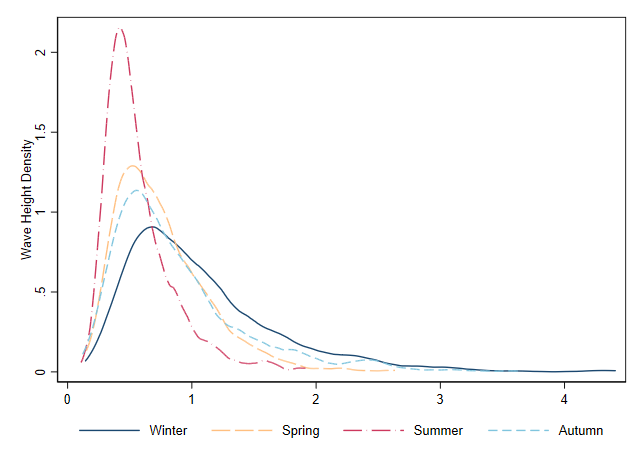
\includegraphics[width=.9\linewidth]{../graphs/figC5}
	\floatfoot*{\footnotesize Note: We gather the data on significant wave height from the European Centre for Medium-Range Weather Forecasts (ECMWF). The density functions show the wave conditions by seasons in Tripoli.}
\end{figure}

%%%%%%%%%%%%%%%%%%%%%%%%%%%%%%%%%%%%%%%%%%%%%%%%%%%%%%%%%%%%%%%%%%%%%%%%%%%%%%%%%%%%%%%%%%%%%%%%%%%%%%%%%%%%%%%%%%%%%
\clearpage
\begin{figure}[th!]\centering
	\RawCaption{\caption{A Typical Inflatable Boat}\label{alibaba}}
	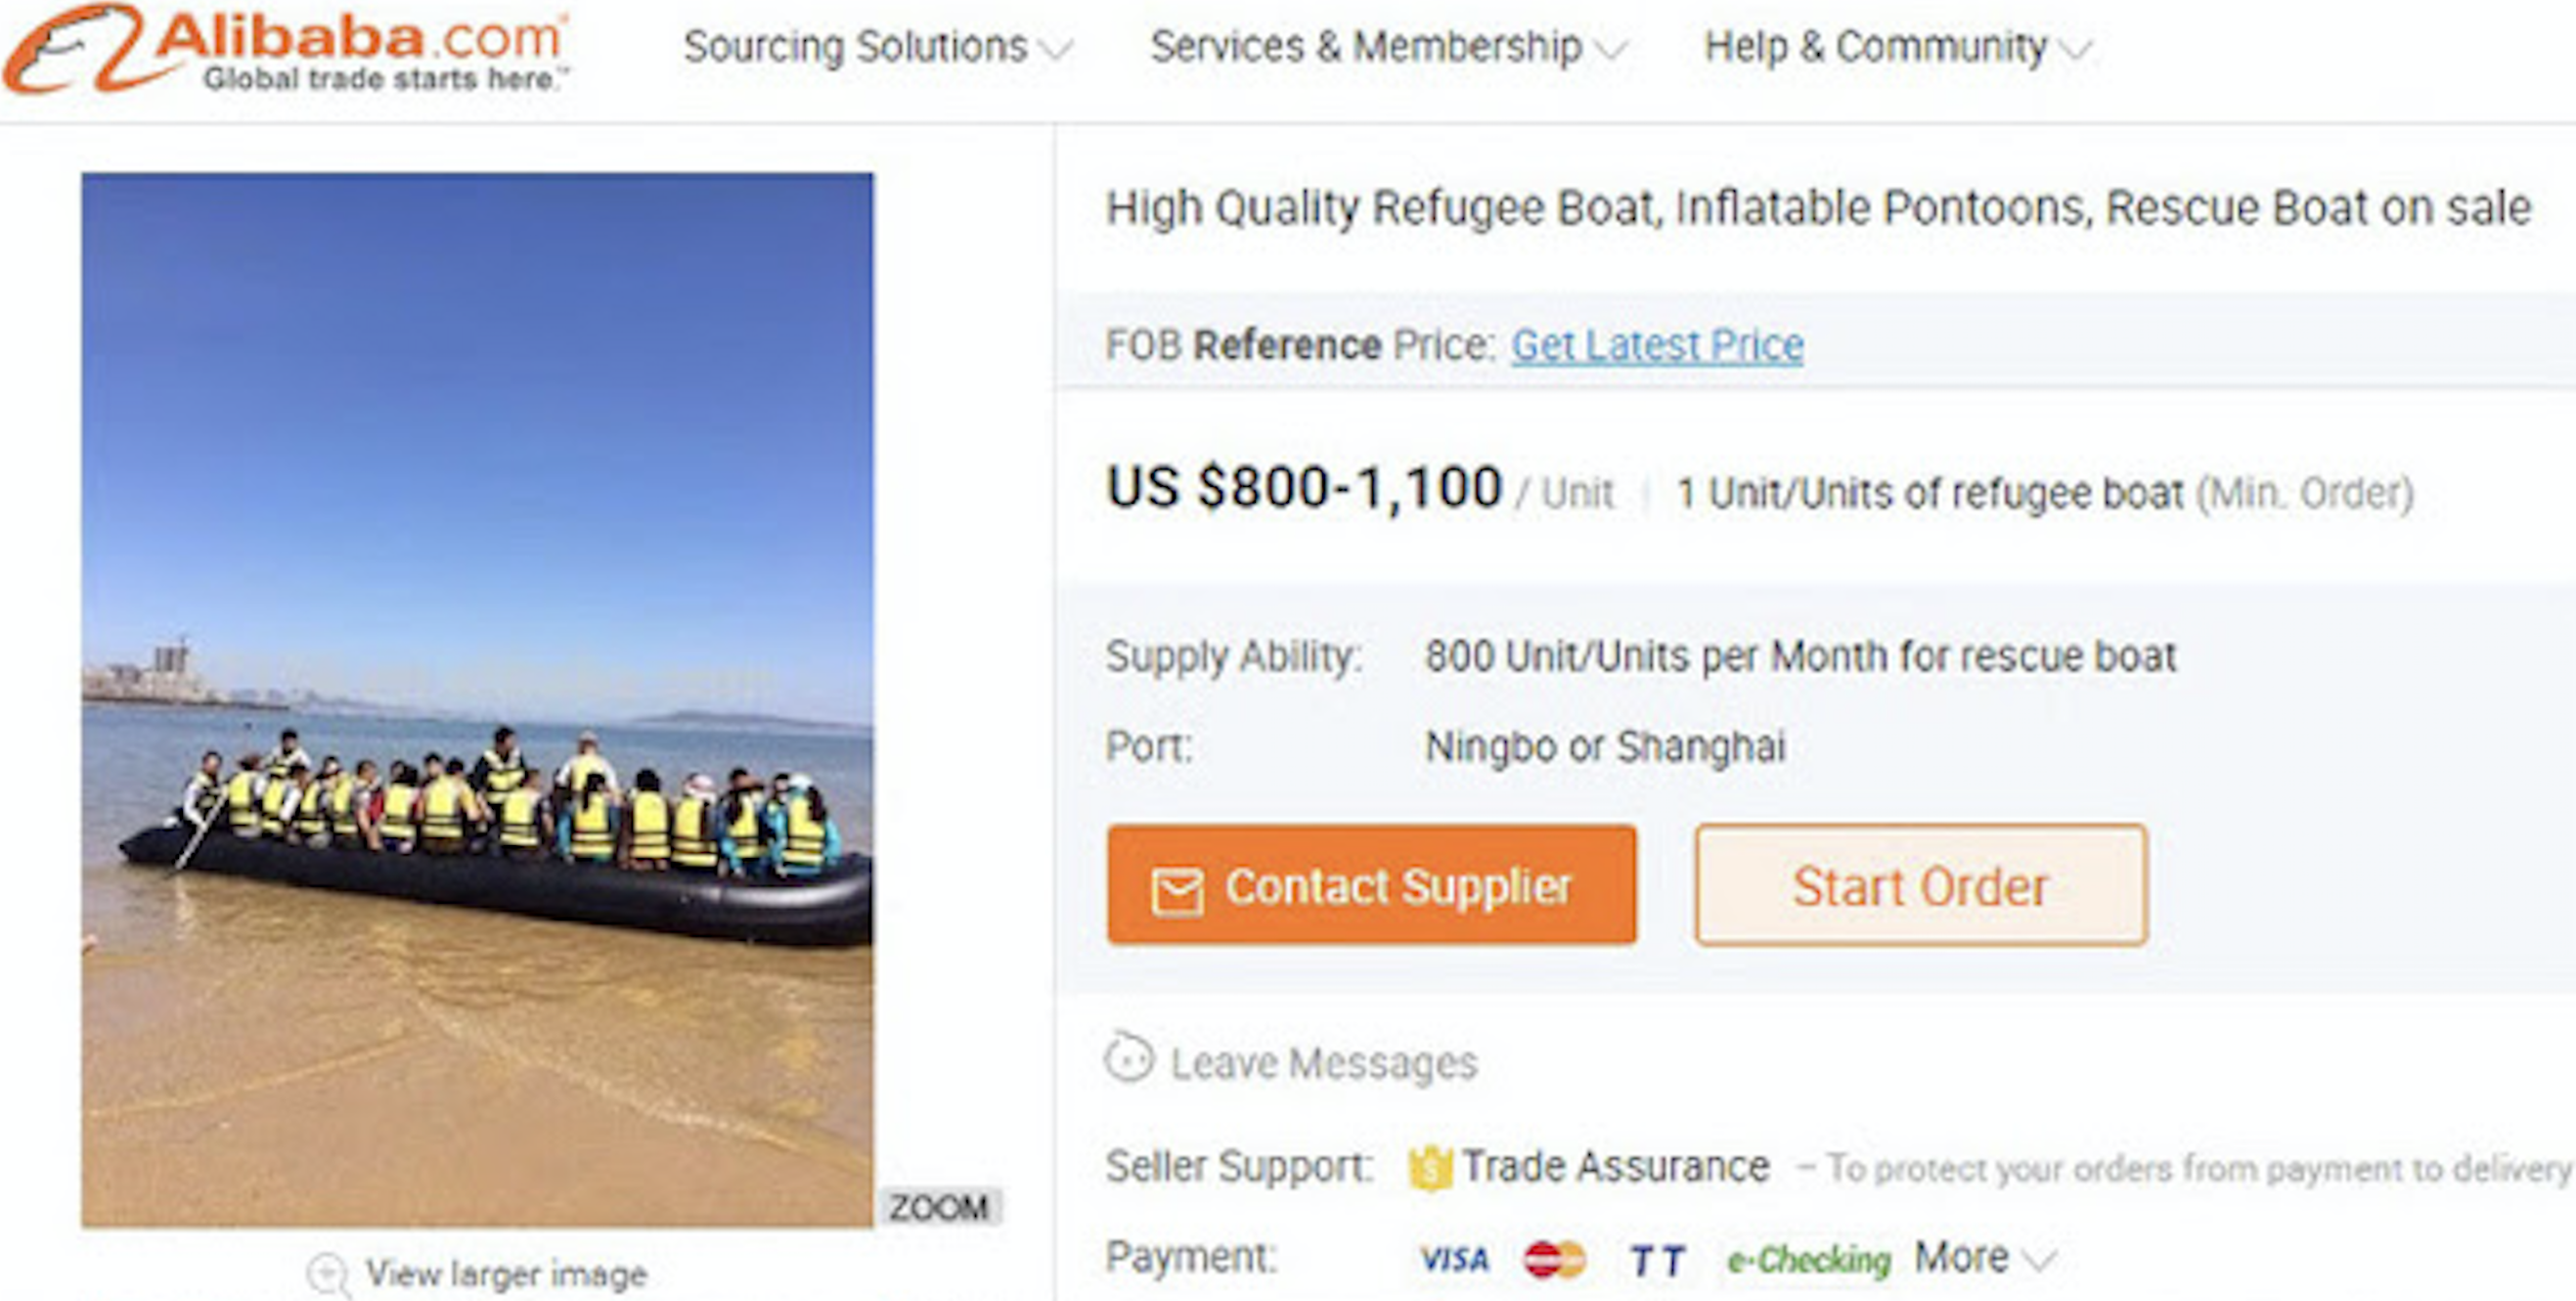
\includegraphics[width=1\linewidth]{../graphs/alibaba_china}
	\flushleft
	\footnotesize{Note: The figure is taken from \url{https://www.alibaba.com} where Chinese-made dinghies were advertised as ``refugee boats'' and  were transshipped to Libya through other countries, i.e. Malta and Turkey.}
\end{figure}


%%%%%%%%%%%%%%%%%%%%%%%%%%%%%%%%%%%%%%%%%%%%%%%%%%%%%%%%%%%%%%%%%%%%%%%%%%%%%%%%%%%%%%%%%%%%%%%%%%%%%%%%%%%%%%%%%%%%%
\clearpage
\begin{figure}[th!]\centering
	\RawCaption{\caption{Probability of Encountering Large Waves}\label{fig:large_waves}}
	\includegraphics[width=.75\linewidth]{../graphs/wave_graph.png}
	\floatfoot*{\footnotesize Note: The figure shows the probability of encountering waves up to ``Wave Height'' when the significant wave height is either 0.63 or 0.73 meters, as well as the corresponding relative difference.}
\end{figure}


%%%%%%%%%%%%%%%%%%%%%%%%%%%%%%%%%%%%%%%%%%%%%%%%%%%%%%%%%%%%%%%%%%%%%%%%%%%%%%%%%%%%%%%%%%%%%%%%%%%%%%%%%%%%%%%%%%%%%
\clearpage
\begin{figure}[th!]\centering
	\RawCaption{\caption{Randomization Inference Using Former Wave Conditions}\label{fig:placi}}
	\begin{tabular}{cc}
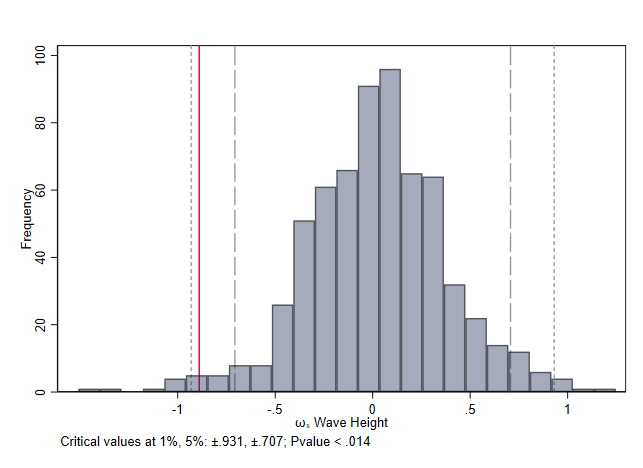
\includegraphics[width=.5\linewidth]{../graphs/figC8a.png}
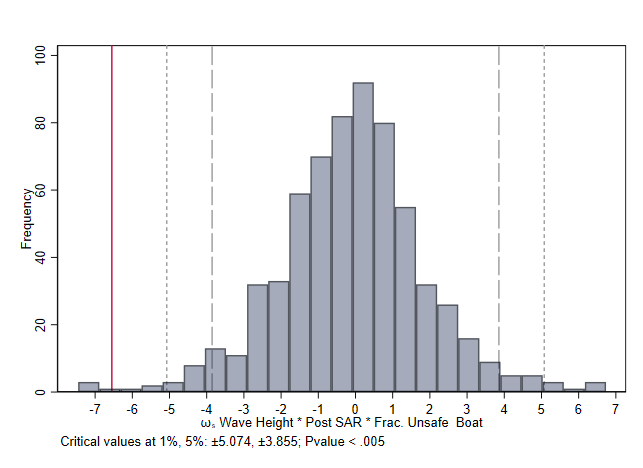
\includegraphics[width=.5\linewidth]{../graphs/figC8b.png}	
\\
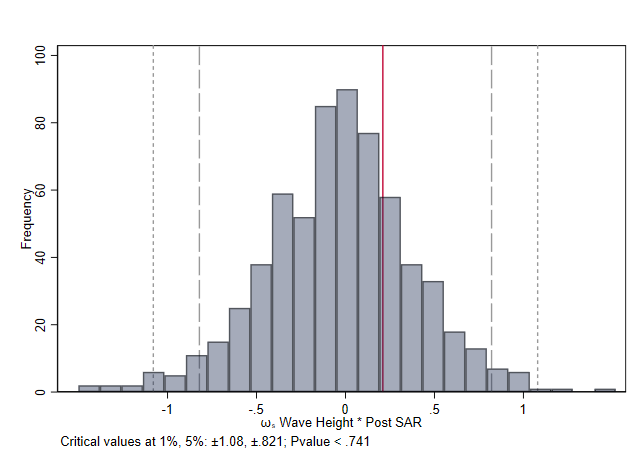
\includegraphics[width=.5\linewidth]{../graphs/figC8c.png}	
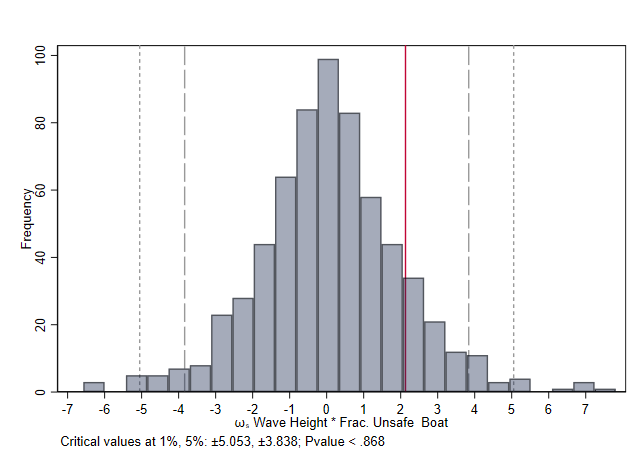
\includegraphics[width=.5\linewidth]{../graphs/figC8d.png}		
	\end{tabular}
	\floatfoot*{\footnotesize Note: The sample consists of daily observations from 7 May 2013 to 4 October 2017. SAR coefficients are estimated relative to a baseline in which Hermes operations (single boat type regime) were in place (164 days). Post SAR dummy is equal to one for all observations after October 18, 2013 (the beginning of the intense SAR when multiple types of boats were used).   Crossing attempts sum crossings and deaths in transit. Significant wave height in Tripoli (Libya) is measured in meters.  We estimate Equation \ref{ppml} 644 times, using wave height at time $t-k$ instead of time $t$, with $k$ ranging from 28 to 672 days. Frac. Unsafe Boat measures the share of attempted crossings using unsafe boats aggregated at the week-year level, i.e. the share of crossing attempts using ``inflatable'' rubber boats over the total. All regressions control for week-by-year fixed effects. Left-top panel shows the placebo for the coefficients of the wave height, right-top panel the triple interaction terms between Frac. Unsafe Boat, post Mare Nostrum period and the wave height in Tripoli. Left-bottom panel shows the placebo for the coefficients of the interaction between wave height in Tripoli and Post SAR, right-bottom panel the double interaction terms between Frac. Unsafe Boat and the wave height in Tripoli. Regressions are estimated using Poisson quasi-maximum likelihood models. The solid red line indicates the estimated coefficients, while the dotted and dashed line indicate the 1\% and 5\% critical values (computed based on the estimated standard deviation).
	}
\end{figure}


%%%%%%%%%%%%%%%%%%%%%%%%%%%%%%%%%%%%%%%%%%%%%%%%%%%%%%%%%%%%%%%%%%%%%%%%%%%%%%%%%%%%%%%%%%%%%%%%%%%%%%%%%%%%%%%%%%%%%
\clearpage
\begin{figure}[th!]\centering
	\RawCaption{\caption{Randomization Inference Using Future Waves}\label{fig:plac_future}}
	\begin{tabular}{cc}
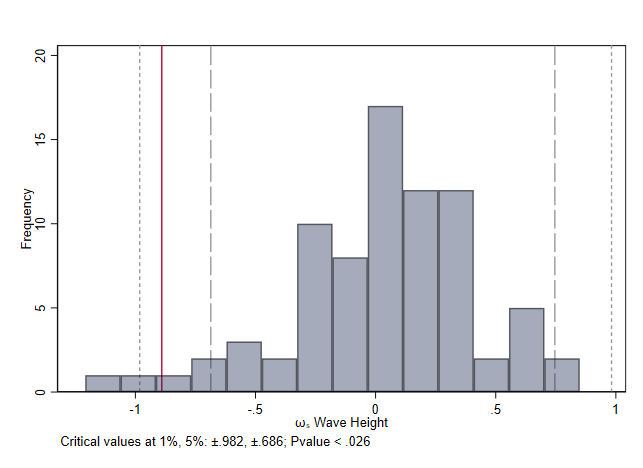
\includegraphics[width=.5\linewidth]{../graphs/figC9a.png}
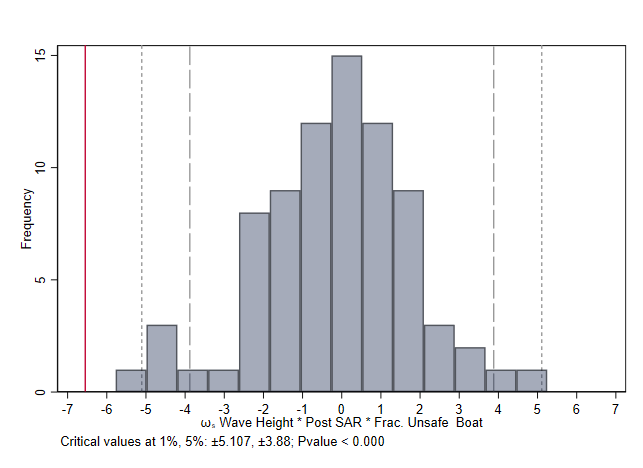
\includegraphics[width=.5\linewidth]{../graphs/figC9b.png}	
\\
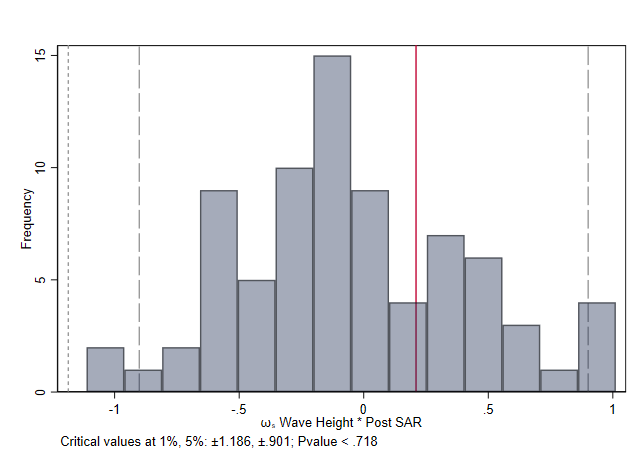
\includegraphics[width=.5\linewidth]{../graphs/figC9c.png}	
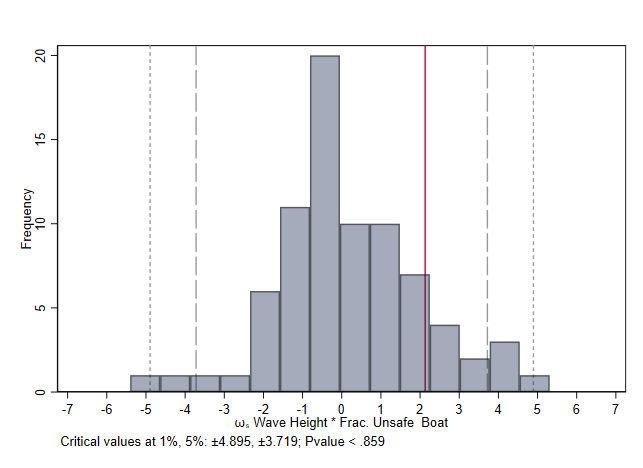
\includegraphics[width=.5\linewidth]{../graphs/figC9d.png}	
	\end{tabular}
	\floatfoot*{\footnotesize Note: The sample consists of daily observations from 7 May 2013 to 4 October 2017. SAR coefficients are estimated relative to a baseline in which Hermes operations (single boat type regime) were in place (164 days). Post SAR dummy is equal to one for all observations after October 18, 2013 (the beginning of the intense SAR when multiple types of boats were used).   Crossing attempts sum crossings and deaths in transit. Significant wave height in Tripoli (Libya) is measured in meters.  We estimate Equation \ref{ppml} 80 times, using wave height at time $t+k$ instead of time $t$, with $k$ ranging from 7 to 87 days. Frac. Unsafe Boat measures the share of attempted crossings using unsafe boats aggregated at the week-year level, i.e. the share of crossing attempts using ``inflatable'' rubber boats over the total. All regressions control for week-by-year fixed effects. Left-top panel shows the placebo for the coefficients of the wave height, right-top panel the triple interaction terms between Frac. Unsafe Boat, post Mare Nostrum period and the wave height in Tripoli. Left-bottom panel shows the placebo for the coefficients of the interaction between wave height in Tripoli and Post SAR, right-bottom panel the double interaction terms between Frac. Unsafe Boat and the wave height in Tripoli. Regressions are estimated using Poisson quasi-maximum likelihood models. The solid red line indicates the estimated coefficients, while the dotted and dashed line indicate the 1\% and 5\% critical values (computed based on the estimated standard deviation).
	}
\end{figure}

%%%%%%%%%%%%%%%%%%%%%%%%%%%%%%%%%%%%%%%%%%%%%%%%%%%%%%%%%%%%%%%%%%%%%%%%%%%%%%%%%%%%%%%%%%%%%%%%%%%%%%%%%%%%%%%%%%%%%
\clearpage
\begin{figure}[th!]\centering
\RawCaption{\caption{Crossing Attempts to Crossing Conditions along Fraction of Unsafe Boats}\label{fig:distr}}
\begin{tabular}{cc}
		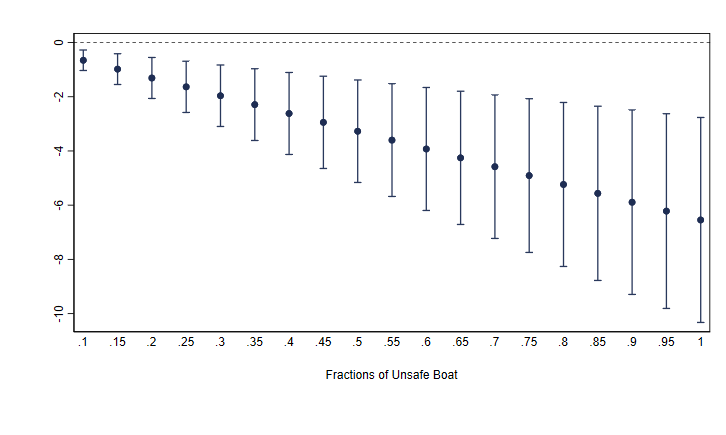
\includegraphics[width=.9\linewidth]{../graphs/figC10.png}
\end{tabular}
\floatfoot{\footnotesize Note: The sample consists of daily observations from 7 May 2013 to 4 October 2017. SAR coefficients are estimated relative to a baseline in which Hermes operations (single boat type regime) were in place (164 days). Post SAR dummy is equal to one for all observations after October 18, 2013 (the beginning of the intense SAR when multiple types of boats were used).  Crossing attempts sum crossings and deaths in transit. Significant wave height in Tripoli (Libya) is measured in meters. Frac. Unsafe Boat measures the share of attempted crossings using unsafe boats aggregated at the week-year level. We use the unsafe boats defined as the share of crossing attempts using ``inflatable'' rubber boats over the total. We provide the estimate of semi-elasticity along different fractions of unsafe boat. All regressions control for week-by-year fixed effects. Regressions are estimated using Poisson quasi-maximum likelihood models. Standard errors are heteroscedasticity- and autocorrelation-robust using Newey-West with a bandwidth equal to 28 days (5\% confidence interval).}
\end{figure}


%%%%%%%%%%%%%%%%%%%%%%%%%%%%%%%%%%%%%%%%%%%%%%%%%%%%%%%%%%%%%%%%%%%%%%%%%%%%%%%%%%%%%%%%%%%%%%%%%%%%%%%%%%%%%%%%%%%%%
\clearpage
\begin{figure}[th!]\centering
	\RawCaption{\caption{Event Study around the Minniti Code}\label{fig:eventdid}}
	\begin{tabular}{cc}
		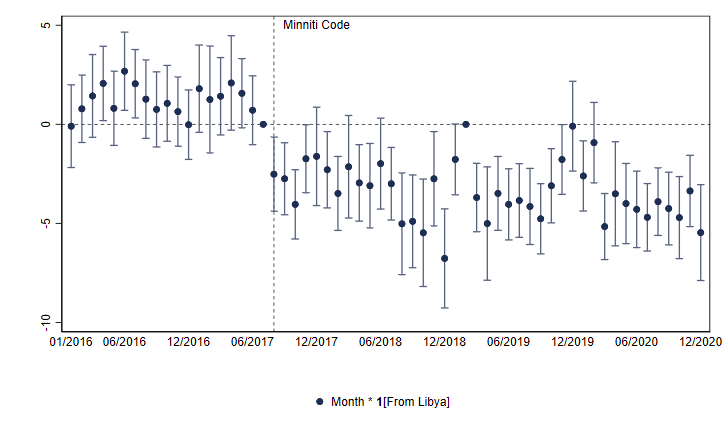
\includegraphics[width=.9\linewidth]{../graphs/figC11.png}
	\end{tabular}
\floatfoot{\footnotesize Note: The sample consists of daily observations from 1 January 2016 to 31 December 2020. SAR dummy is equal to one for all observations before August 7, 2017, when multiple boat types were used more frequently. This corresponds to pre-\emph{Minniti} periods, i.e.~before the Code of Conduct was enacted restricting \textit{de-facto} the use of unsafe boats. The Libyan route is considered as treated unit. Time indicate the month of the year. Crossing attempts sum crossings and deaths. All regressions control for week-by-year fixed effects. In February 2019 no crossing attempts occurred so no coefficient is estimated (it is absorbed by week-by-year fixed effects). Regressions estimated using Poisson quasi-maximum likelihood models. Figure shows the dynamic effect of the main result in Table \ref{tab:did}, i.e. the interaction between $Wave \: Height * From \: Libya * Frac. \: Inflatable \: Boat * SAR$. Each coefficient represents the interaction between the dummy-month of the year and the treatment, i.e. if the crossings attempts come from Libya. Baseline period is July, 2017. Standard errors are cluster at the week of the year level. (5\% confidence interval).}
\end{figure}




%%%%%%%%%%%%%%%%%%%%%%%%%%%%%%%%%%%%%%%%%%%%%%%%%%%%%%%%%%%%%%%%%%%%%%%%%%%%%%%%%%%%%%%%%%%%%%%%%%%%%%%%%%%%%%%%%%%%%
\clearpage
\section*{Appendix D: NGO Operations (For Online Publication Only)}\label{s:NGO}
\setcounter{subsection}{0} 	
\renewcommand{\thesubsection}{D.\arabic{subsection}}
\setcounter{figure}{0} 		
\renewcommand{\thefigure}{D.\arabic{figure}}
\setcounter{table}{0}  		
\renewcommand{\thetable}{D.\arabic{table}}

\begin{table}[bh!]\small 
	\RawCaption{\caption{NGO Vessels and Operational Period}\label{tab:listNGO}}
	\floatbox[{\captop}]{table}[\FBwidth]
	{}
	{\resizebox{\textwidth}{!}{\begin{tabular}{L{5.5cm}L{5cm}L{4cm}L{3cm}L{4cm}}
\toprule\toprule
NGO                           & Country                    & Flag               & Vessel        & Operational Period               \\
\hline
&&&& \\
Jugend Rettet                  & Germany                    & The Netherlands    & Iuventa       & Jul 2016 - Nov 2016 \\
LifeBoat                       & Germany                    & Germany            & Minden        & Jun 2016 - Nov 2016 \\
Médecins Sans Frontières (MSF) & France                     & Italy              & Vos Prudence  & Mar 2017 - Oct 2017 \\
Médecins Sans Frontières (MSF) & France                     & Panama             & Dignity I     & May 2015 - Dec 2016 \\
Médecins Sans Frontières (MSF) & France                     & Luxembourg         & Bourbon-Argos & May 2015 - Nov 2016 \\
ProActiva Open Arms            & Spagna                     & Panama             & Golfo Azzurro & Dec 2016 - Sep 2017  \\
ProActiva Open Arms            & Spagna                     & The United Kingdom & Astral        & Jun 2016 - Nov 2016 \\
Save the Children              & International Organization & Italy              & Vos Hestia    & Sep 2016 - Nov 2016 \\
Sea-Watch                      & Germany                    & Germany            & Sea-Watch     & Jun 2015 - Nov 2016 \\
Sea-Watch                      & Germany                    & The Netherlands    & Sea-Watch 2   & Mar 2016 - Nov 2016 \\
Sea-Eye                        & Germany                    & The Netherlands    & Sea-Eye       & Feb 2016 - Nov 2016 \\
SOS Méditerranée               & France-Italy-Germany       & Gibraltar          & Aquarius      & Feb 2016 - Dec 2016 \\
\bottomrule\bottomrule
\end{tabular}%

			\floatfoot*{\footnotesize Source: The list of NGOs operating in the Mediterranean Sea is available in the Italian Navy report (\citeyear{EUNAVFOR_2017}). The table distinguishes between the country and flag of the boat, the vessel type and the operational period.}
	}}
\end{table}



\clearpage
\begin{figure}[bh!]\centering
	\RawCaption{\caption{Rescue Activity by Organization 2014-2017}\label{eu_ngo_attempt2}}	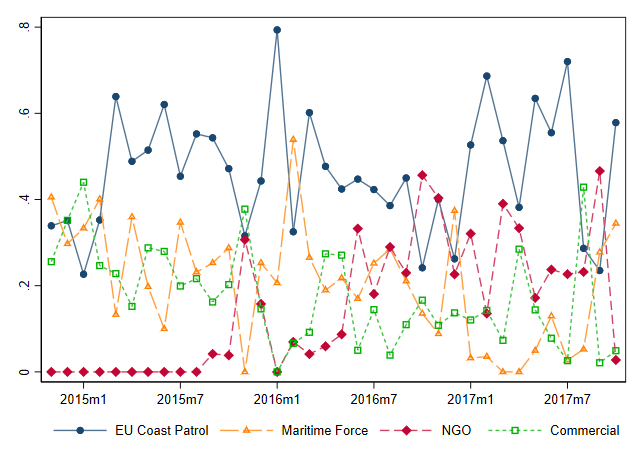
\includegraphics[width=.75\linewidth]{../graphs/figD1}
	\floatfoot*{\footnotesize Note: Data provided by the European Border and Coast Guard Agency known as Frontex. The information is disclosed by Frontex for the period from January, 2015 to December, 2017. Each line represents the fraction of monthly crossings that are intercepted by any given organization (EU coast patrol, Maritime force, NGOs and Commercial boats). Their sum is always one.}	
\end{figure}


\end{document}
